\documentclass[a4paper,12pt]{article}

%%% Работа с русским языком

\usepackage{cmap}					% поиск в PDF
\usepackage{mathtext} 				% русские буквы в формулах
\usepackage[T2A]{fontenc}			% кодировка
\usepackage[utf8]{inputenc}			% кодировка исходного текста
\usepackage[english,russian]{babel}	% локализация и переносы
\usepackage{indentfirst}            % красная строка в первом абзаце
\usepackage[unicode]{hyperref}
\usepackage{epigraph}
\frenchspacing                      % равные пробелы между словами и предложениями

%%% Дополнительная работа с математикой
\usepackage{amsmath,amsfonts,amssymb,amsthm,mathtools} % пакеты AMS
\usepackage{bbm} % Blackboard bold для цифр
\usepackage{icomma}                                    % "Умная" запятая

\renewcommand{\phi}{\ensuremath{\varphi}}
\renewcommand{\kappa}{\ensuremath{\varkappa}}
\renewcommand{\le}{\ensuremath{\leqslant}}
\renewcommand{\leq}{\ensuremath{\leqslant}}
\renewcommand{\ge}{\ensuremath{\geqslant}}
\renewcommand{\geq}{\ensuremath{\geqslant}}
\renewcommand{\emptyset}{\ensuremath{\varnothing}}

\newcommand{\cl}{\text{cl }}
\newcommand{\setint}{\text{int }}

\theoremstyle{plain}
\newtheorem{theorem}{Теорема}[section]
\newtheorem{lemma}{Лемма}[section]
\newtheorem{proposition}{Утверждение}[section]
\newtheorem*{corollary}{Следствие}
\newtheorem*{exercise}{Упражнение}

\theoremstyle{definition}
\newtheorem{definition}{Определение}[section]
\newtheorem*{note}{Замечание}
\newtheorem*{reminder}{Напоминание}
\newtheorem*{example}{Пример}
\newtheorem*{tasks}{Вопросы и задачи}

\theoremstyle{remark}
\newtheorem*{solution}{Решение}

%%% Оформление страницы
\usepackage{extsizes}     % Возможность сделать 14-й шрифт
\usepackage{geometry}     % Простой способ задавать поля
\usepackage{setspace}     % Интерлиньяж
\usepackage{enumitem}     % Настройка окружений itemize и enumerate
\usepackage{epigraph}     % Эпиграф
\setlist{leftmargin=25pt} % Отступы в itemize и enumerate

\geometry{top=25mm}    % Поля сверху страницы
\geometry{bottom=30mm} % Поля снизу страницы
\geometry{left=20mm}   % Поля слева страницы
\geometry{right=20mm}  % Поля справа страницы

\begin{document}
\tableofcontents
\newpage

\section{Теорема Римана об осцилляции}

\epigraph{Порядок и беспорядок – это число; храбрость и трусость – это мощь; сила и слабость – это форма.}{Лукашов А.Л.}

\begin{definition}
	Точка $x$ называется \textbf{точкой прикосновения} множества $S$, если любая окресность $x$ содержит хотя бы одну точку множества $S$.
\end{definition}

\begin{definition}
	Множество всех точек прикоcновения $S$ называется \textbf{замыканием} $S$.
\end{definition}

\begin{definition}
	\textbf{Носителем} функции $f(x)$ называется замыкание множества тех $x$, для которых $f(x) \neq 0$. (supp $f$) Функции с ограниченным носителем называются \textbf{финитными}.
\end{definition}

\begin{definition}
	Множество $D$ называется всюду плотным в множестве $G$, если
	\[\overline{D} = G\]
\end{definition}

\begin{proposition}
	$L_1(\mathbb{R})$ -- линейное нормированное пространство.
	\[\|f\|_1 = \int_\mathbb{R} |f(x)| d\mu(x)\]
\end{proposition}

\begin{lemma}
	\label{C_IN_PLOTNI}

	Множество непрерывных финитных функций всюду плотно в $L_1(\mathbb{R})$.
\end{lemma}

\begin{proof}
	Заменим $\mathbb{R}$ на $[a,\,b]$. То есть докажем, что множество непрерывных на $[a,\,b]$ функций всюду плотно в $L_1[a,\,b]$.

	\begin{itemize}
		\item Любая суммируемая функция представима в виде разности двух неотрицательных суммируемых функций, поэтому достаточно доказать утверждение для
		      неотрицательных суммируемых функций.
		\item Так как интеграл неотрицательной суммируемой функции слабо отличается от интеграла её срезки $f_{[N]}(x)$ при достаточно больших $N$, то
		      достаточно доказать утверждение для ограниченных неотрицательных суммируемых функций.
		\item Докажем для ограниченных неотрицательных. По теореме о представлении ограниченной измеримой функции пределом последовательности ступенчатых
		      \[\exists \{h_n\}_{n = 1}^\infty:\: h_n \uparrow f\]
		      Теорема Леви гарантирует, что
		      \[\int_a^b h_n(x)d\mu(x) \to \int_a^b f(x)d\mu(x)\]
		      Значит
		      \begin{align*}
			      \int_a^b |f(x) - h_n(x)|d\mu(x) = \int_a^b (f(x) - h_n(x))d\mu(x) \stackrel{n \to +\infty}{\to} 0
		      \end{align*}
		      То есть нам достаточно доказать, что любую ступенчатую можно приблизить непрерывной:
		      \[h_n(x) = \sum_{k = 1}^N c_k \mathbb{I}_{E_k}(x)\]
		      В силу того, что $\forall k:\: E_k$ -- измеримое, то
		      \[\forall \varepsilon > 0:\: \exists \text{элементарное } M_\varepsilon:\: \mu(E_k \triangle M_\varepsilon) < \varepsilon \]
		      Значит
		      \[\int_a^b |\mathbb{I}_{E_k}(x) - \mathbb{I}_{M_\varepsilon}(x)|d\mu(x) = \int_a^b \mathbb{I}_{E \triangle M_\varepsilon}(x)d\mu(x) = \mu(E \triangle M_\varepsilon) < \varepsilon\]
		      Нам осталось научиться приближать индикатор интервала непрерывными функциями (так как элементарное множество представимо объединением интервалов), а это сделать очень просто, используя непрерывную функцию $\phi(x)$, которая выглядит вот так:
		      \begin{figure}[h]
			      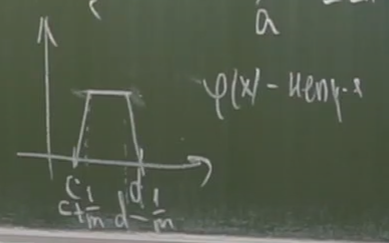
\includegraphics[scale=0.5]{img/phi_graph.png}
			      \caption{Один из способов ввода функции $\phi$}
		      \end{figure}

		      Тогда
		      \[\int_a^b |\mathbb{I}_{(c,\,d)}(x) - \phi(x)|d\mu(x) = \frac{2}{m} < \varepsilon\]
	\end{itemize}

	Возвращаемся к общему случаю: пусть $f \in L_1(\mathbb{R})$.

	\[\exists N \in \mathbb{N}\: \int_{\mathbb{R} \setminus [-N,\,N]}|f(x)|d\mu(x) < \frac{\varepsilon}{3}\]
	По доказанному выше:
	\[f|_{[-N,\,N]} :\: \forall \varepsilon > 0 \:\exists g \in C[-N,\,N] \: \|f|_{[-N,\,N]} - g\|_{L_1[-N,\,N]} < \frac{\varepsilon}{3}\]
	Далее мы можем продлить $g$ на всю прямую линейным образом (аналогично введению функции $\phi$ из рассуждений выше), так, чтобы
	\[\int_{\mathbb{R}\setminus [-N,\,N]} |g(x)|d\mu(x) < \frac{\varepsilon}{3}\]
	Тогда
	\[\int_\mathbb{R} |f(x) - g(x)|d\mu(x) \leq \int_{-N}^N |f(x) - g(x)|d\mu(x) + \int_{\mathbb{R} \setminus [-N,\,N]} (|f(x)| + |g(x)|) d\mu(x) < \varepsilon\]
\end{proof}

\begin{lemma}
	\label{CONT_MODUL}

	Каждая суммируемая на $\mathbb{R}$ функция $f(x)$ непрерывна в среднем относительно сдвига, то есть
	\[\lim_{t \to 0} \int_\mathbb{R} |f(x + t) - f(x)| d\mu(x) = 0\]
\end{lemma}

\begin{proof}
	Докажем, что для $f \in L_1[a,\,b]$:
	\[\lim_{\delta \to +0} \sup_{0 \leq h \leq \delta} \int_a^{b - h} |f(x + h) - f(x)|d\mu(x) = 0\]
	По предыдущей лемме:
	\[\forall \varepsilon > 0 \: \exists g \in C[a,\,b]:\: \int_a^b |f(x) - g(x)|d\mu(x) < \frac{\varepsilon}{3}\]
	$g$ -- непрерывная на $[a,\,b] \Rightarrow$ по теореме Кантора она равномерно непрерывная на $[a,\,b]$:
	\[\forall \varepsilon > 0 \: \exists \delta > 0 \: \forall x,\,y \in [a,\,b],\, |x - y| < \delta :\: |g(x) - g(y)| < \frac{\varepsilon}{3(b - a)}\]
	Тогда $\forall h \: 0 \leq h \leq \delta$:
	\begin{align*}
		\int_a^{b - h}|f(x + h) - f(x)|d\mu(x) \leq \int_a^{b - h} |f(x + h) - g(x + h)|d\mu(x) + \int_a^{b - h}|f(x) - g(x)|d\mu(x) + \\
		+ \int_a^{b - h}|g(x + h) - g(x)|d\mu(x) < \varepsilon
	\end{align*}
	Так как $f$ суммируема на $\mathbb{R}$, то $\exists N \in \mathbb{N}$:
	\[\int_{\mathbb{R} \setminus [-N,\,N]}|f(x)|d\mu(x) < \frac{\varepsilon}{3}\]
	Тогда выберем $[a,\,b] := [-N - 1,\,N + 1]$ и введём $g := f\mathbb{I}_{[-N,\,N]} \in L_1[a,\,b]$. Применим к этой функции доказанное выше равенство:
	\[\exists \delta \in (0,\,1) \: \forall h,\, 0 \leq h \leq \delta :\: \int_a^{b - h}|g(x + h) - g(x)|d\mu(x) < \frac{\varepsilon}{3}\]
	Теперь возьмём $\forall t,\, |t| < \delta$:
	\[
		\int_\mathbb{R}|f(x + t) - f(x)|d\mu(x) = \int\limits_{\{x,\,x+t\}\subseteq[a,\,b]}|f(x+t)-f(x)|d\mu(x) + \int\limits_{\{x,\,x+t\}\not\subseteq[a,\,b]}|f(x+t)-f(x)|d\mu(x) < \varepsilon
	\]
\end{proof}

\begin{theorem}
	Римана об осцилляции.

	Если $f \in L_1(I)$, где $I$ -- конечный или бесконечный промежуток, то
	\[\lim_{\lambda \to \infty} \int_I f(x)\cos(\lambda x) d \mu(x) = \lim_{\lambda \to \infty} \int_I f(x) \sin (\lambda x) d\mu(x) = 0\]
\end{theorem}

\begin{proof}
	\begin{align*}
		\int_I f(x) \cos(\lambda x) d\mu(x) \stackrel{x = t + \frac{\pi}{\lambda}}{=} - \int_{I - \frac{\pi}{\lambda}} f\left( t + \frac{\pi}{\lambda} \right) \cos(\lambda t) d \mu(t) = \\
		-\frac{1}{2} \int_I \left(f\left(t + \frac{\pi}{\lambda}\right) - f(t) \right)\cos(\lambda t) d\mu(t) - \frac{1}{2} \int_{(I - \frac{\pi}{\lambda}) \triangle I} f\left(t + \frac{\pi}{\lambda}\right) \cos(\lambda t) d \mu(t)
	\end{align*}
	Заметим, что
	\begin{align*}
		\left|\int_{(I - \frac{\pi}{\lambda}) \setminus I} f\left(t + \frac{\pi}{\lambda}\right) \cos(\lambda t) d \mu(t)\right| \leq \int_{(I - \frac{\pi}{\lambda}) \triangle I} \left|f\left(t + \frac{\pi}{\lambda}\right)\right| d\mu(t) = \\
		= \int_{I \triangle (I + \frac{\pi}{\lambda})} |f(x)|d\mu(x) \stackrel{\lambda \to \infty}{\to} 0
	\end{align*}
	Последнее заключение следует из того, что $\mu\left(I \triangle (I + \frac{\pi}{\lambda})\right) \stackrel{\lambda \to \infty}{\to} 0$

	Также очевидно, что
	\begin{align*}
		\left|\int_I \left(f\left(t + \frac{\pi}{\lambda}\right) - f(t) \right)\cos(\lambda t) d\mu(t)\right| \leq \int_I \left|f\left(t + \frac{\pi}{\lambda}\right) - f(t)\right|d\mu(t) \stackrel{\text{по пред. Лемме}}{\to} 0
	\end{align*}
\end{proof}

\section{Представление частичной суммы ряда Фурье интегралом с ядром Дирихле. Принцип локализации.}

\epigraph{О мастерстве полководца судят по старательности его подчиненных.}{Лукашов А.Л.}

\begin{definition}
	$f \in L_{2\pi} \Leftrightarrow f \in L_1[-\pi,\,\pi]$ и $2\pi$ периодическая.
\end{definition}

\begin{definition}
	Ядром Дирихле $D_n(u)$ называется выражение
	\[D_n(u) = \frac{1}{2} + \sum_{k = 1}^n \cos(ku) = \frac{\sin (n + \frac{1}{2})u}{2\sin(\frac{u}{2})}\]
\end{definition}

\begin{proof}
	\begin{align*}
		D_n(u) = \frac{1}{2} + \sum_{k = 1}^n \cos(ku) = \frac{1}{2} + \frac{1}{2}\sum_{k = 1}^n (e^{iku} + e^{-iku}) = \frac{1}{2}\sum_{k = -n}^n e^{iku} = \frac{1}{2}e^{-inu}\frac{e^{i(2n + 1)u} - 1}{e^{iu} - 1} = \\
		= \frac{1}{2}e^{-inu}\frac{e^{i(2n + 1)\frac{u}{2}} - e^{-i(2n + 1)\frac{u}{2}}}{e^{i\frac{u}{2}} - e^{-i\frac{u}{2}}}\cdot\frac{e^{i(2n + 1)\frac{u}{2}}}{e^{i\frac{u}{2}}} = \frac{1}{2}\frac{\sin((n + \frac{1}{2})u)}{\sin(\frac{u}{2})}
	\end{align*}
\end{proof}

\begin{lemma}
	О представлении частичной суммы.

	Если $f \in L_{2\pi}$, то $n$-я частичная сумма тригонометрического ряда Фурье
	\[S_n(f,\,x) = \frac{a_0}{2} + \sum_{k = 1}^n (a_k \cos(kx) + b_k\sin(kx))\]
	может быть представлена следующим образом:
	\[S_n(f,\,x) = \frac{1}{\pi}\int_{-\pi}^\pi f(t)D_n(x - t)d\mu(t) = \frac{1}{\pi}\int_{-\pi}^\pi f(x + u)D_n(u)d\mu(u)\]
\end{lemma}

\begin{proof}
	Подставим в $S_n$ формулы для $a_k,\, b_k$:
	\begin{align*}
		S_n(f,\,x) = \frac{1}{\pi}\int_{-\pi}^\pi f(t) \left(\frac{1}{2} + \sum_{k = 1}^n (\cos(kx)\cos(kt) + \sin(kx)\sin(kt))\right)d\mu(t) = \\
		= \frac{1}{\pi}\int_{-\pi}^\pi f(t)D_n(x-t)d\mu(t)
	\end{align*}
	Первая формула доказана, вторая доказывается очевидно заменой $t = x + u$, а также используя тот факт, что интеграл по любому отрезку длины $T$, $T$-периодичной функции одинаков.
\end{proof}

\begin{lemma}
	\label{RAVN_COEF}
	Пусть $f \in L_{2\pi}$, $g$ -- измеримая, $2\pi$-периодическая, ограниченная функция. Тогда коэффициенты Фурье функции $\chi(t) = f(x + t)g(t)$ стремятся к нулю при $n \to +\infty$ равномерно по $x$.
\end{lemma}

\begin{proof}
	$g$ -- ограниченная $\Rightarrow \exists M:\: \forall u \: |g(u)| \leq M$.

	$f$ -- суммируемая $\Rightarrow$ по (\ref{C_IN_PLOTNI}) мы можем её представить, как $f = f_1 + f_2$, причём $f_1 \in C[-\pi,\,\pi]$, а $\int_{-\pi}^{\pi} |f_2(t)|d\mu(t) < \frac{\varepsilon}{4M}$.

	$f_1$ -- непрерывная на компакте $[-\pi,\,\pi] \Rightarrow \exists B \: \forall u:\: |f_1(u)| \leq B$.

	Введём функцию, которая называется интегральный модуль непрерывности функции $F$:
	\[\omega_1(\delta,\,F) := \sup_{0 \leq h \leq \delta} \int_{-\pi}^\pi |F(t + h) - F(t)|d\mu(t)\]
	Рассмотрим $a_n$ для функции $\chi$:
	\begin{align*}
		a_n(\chi) = \frac{1}{\pi} \int_{-\pi}^\pi \chi(t)\cos(nt)d\mu(t) \stackrel{t = u + \frac{\pi}{n}}{=} \frac{-1}{\pi}\int_{-\pi}^\pi \chi\left(u + \frac{\pi}{n}\right)\cos(nu)d\mu(u) = \\
		= \frac{-1}{2\pi}\int_{-\pi}^\pi \left[\chi\left(t + \frac{\pi}{n}\right) - \chi(t)\right]\cos(nt)d\mu(t) \Rightarrow                                                                  \\
		|a_n(\chi)| \leq \frac{1}{2\pi}\omega_1\left(\frac{\pi}{n},\, \chi\right)
	\end{align*}
	Аналогично получим неравенство для $b_n(\chi)$:
	\[|b_n(\chi)| \leq \frac{1}{2\pi}\omega_1\left(\frac{\pi}{n},\,\chi\right)\]
	То есть мы свели доказательство к доказательству факта, что $\lim\limits_{n \to +\infty}\omega_1(\frac{\pi}{n},\,\chi) = 0$ равномерно по $x$:
	\begin{align*}
		\int_{-\pi}^\pi |\chi(t + h) - \chi(t)|d\mu(t) = \int_{-\pi}^\pi |f(x + t + h)g(t + h) - f(x + t)g(t)|d\mu(t) \leq                        \\
		\leq \int_{-\pi}^\pi |f(x + t + h) - f(x + t)|\cdot |g (t + h)|d\mu(t) + \int_{-\pi}^\pi |f(x + t)|\cdot |g(t + h) - g(t)|d\mu(t) \leq    \\
		\leq M \int_{-\pi}^\pi |f(u + h) - f(u)|d\mu(u) +  \int_{-\pi}^\pi |f_1(x + t)|\cdot|g(t + h) - g(t)|d\mu(t) + \frac{\varepsilon}{2} \leq \\
		\leq M \omega_1(\frac{\pi}{n},\, f) + B\omega_1(\frac{\pi}{n},\,g) + \frac{\varepsilon}{2}
	\end{align*}
	Но по (\ref{CONT_MODUL}) мы знаем, что модуль непрерывности стремится к нулю при $\delta \to 0$. Что и требовалось доказать.
\end{proof}

\begin{theorem}
	Принцип локализации.

	Если $f \in L_{2\pi}$ и тождественно равна нулю в некотором интервале $(a,\,b) \subset [-\pi,\,\pi]$, то её тригонометрический ряд Фурье сходится к нулю равномерно на любом отрезке $[a',\,b'] \subset (a,\,b)$.
\end{theorem}

\begin{proof}
	Так как $[a',\,b']$ содержится в $(a,\,b)$, то
	\[\exists \eta > 0 \: \forall x \in [a',\,b'] \: \forall t,\, 0 \leq |t| < \eta :\: x + t \in (a,\,b)\]
	Построим функцию $\lambda(t)$:
	\[
		\lambda(t) = \begin{cases}
			0,\, t \in (-\eta,\,\eta) \\
			1,\, t \in [-\pi,\,\pi]\setminus (-\eta,\,\eta)
		\end{cases}
	\]
	Кроме того, $\lambda$ -- $2\pi$-периодическая.

	Тогда, используя лемму о представлении частичной суммы, получим:
	\[
		S_n(f,\,x) = \frac{1}{\pi}\int_{-\pi}^\pi f(x + t)D_n(t)d\mu(t) = \frac{1}{\pi}\int_{-\pi}^\pi f(x + t)\lambda(t)D_n(t)d\mu(t)
	\]
	Данное соотношение верно, так как когда $t \not\in (-\eta,\,\eta)$, то $\lambda(\eta) = 1$, ничего не меняем. Если же $|t| < \eta$, то $x + t \in (a,\,b)$, где $f = 0$, поэтому получили, что подыинтегральные функции совпадают везде на $[-\pi,\,\pi]$.

	Продолжим раскрытия данной формулы, используя тригонометрические соотношения для ядра Дирихле:
	\begin{align*}
		S_n(f,\,x) = \frac{1}{\pi}\int_{-\pi}^\pi f(x + t)\lambda(t)\ctg\left(\frac{t}{2}\right)\sin(nt)d\mu(t) + \frac{1}{2\pi}\int_{-\pi}^\pi f(x+t)\lambda(t)\cos(nt)d\mu(t)
	\end{align*}
	Взяв в качестве $g$ из предыдущей леммы для первого слагаемого $\lambda(t)\ctg(\frac{t}{2})$ и $\lambda(t)$ для второго, то получим требуемое по этой же лемме.

\end{proof}

\section{Достаточные условия сходимости ряда Фурье в точке}

\epigraph{Одержать сто побед в ста битвах — это не вершина воинского искусства. Повергнуть врага без сражения — вот вершина.}{Лукашов А.Л.}

\begin{theorem}
	Признак Дини.

	Если $f \in L_{2\pi}$ и $\phi_{x_0} \in L_1(0,\,\delta),\, \delta > 0$, где
	\[\phi_{x_0}(t) := \frac{f(x_0 + t) + f(x_0 - t) - 2S(x_0)}{t}\]
	то тригонометрический ряд Фурье функции $f(x)$ сходится к $S(x_0)$.
\end{theorem}

\begin{proof}
	Рассмотрим разность $S_n(f,\,x_0) - S(x_0)$, пользуясь леммой о представлении, можем записать её как
	\[S_n(f,\,x_0) - S(x_0) = \frac{1}{\pi}\int_{0}^\pi (f(x + u) + f(x - u) - 2S(x_0)) D_n(u)d\mu(u)\]
	В данном представлении мы воспользовались сразу несколькими фактами:
	\begin{itemize}
		\item Подынтегральная функция чётная относительно $u$
		\item Интеграл по $[-\pi,\,\pi]$ от ядра Дирихле равен $\pi$
		\item Если заменить в представлении частичной суммы $t$ на $-t$, то ничего не изменится
	\end{itemize}
	Продолжим цепочку преобразований, раскрыв $\sin((n + \frac{1}{2})t) = \sin(nt)\cos(\frac{t}{2}) + \cos(nt)\sin(\frac{t}{2})$ в формуле ядра Дирихле, а также добавим и вычтем интеграл $\frac{1}{\pi} \int_0^\delta \frac{f(x + t) + f(x - t) - 2S(x_0)}{t} \sin(nt)d\mu(t)$:
	\begin{align*}
		S_n(f,\,x_0) - S(x_0) =                                                                                                   \\
		\frac{1}{\pi} \int_0^\delta \frac{f(x + t) + f(x - t) - 2S(x_0)}{t} \sin(nt)d\mu(t) +                                     \\
		\frac{1}{\pi}\int_0^\pi (f(x + t) + f(x - t) - 2S(x_0))\frac{\cos(nt)}{2}d\mu(t) +                                        \\
		\frac{1}{\pi}\int_\delta^\pi (f(x + t) + f(x - t) - 2S(x_0))\frac{\sin(nt)\cos(\frac{t}{2})}{2\sin(\frac{t}{2})}d\mu(t) + \\
		\frac{1}{\pi}\int_0^\delta (f(x + t) + f(x - t) - 2S(x_0))\sin(nt) \left(\frac{\cos(\frac{t}{2})}{2\sin(\frac{t}{2})} - \frac{1}{t}\right)d\mu(t)
	\end{align*}
	По условию, $\phi_{x_0}$ суммируемая $\Rightarrow$ по теореме Римана об осцилляции первое слагаемое стремится к нулю.

	$(f(x + t) + f(x-t) - 2S(x_0))$ также суммируемая $\Rightarrow$ второе слагаемое тоже стремится к нулю.

	В третьем слагаемом $(f(x + t) + f(x - t) - 2S(x_0))\frac{\cos(\frac{t}{2})}{2\sin(\frac{t}{2})} \in L_1[\delta,\,\pi]$ и по той же причине стремится к нулю.

	Для четвёртого слагаемого рассмотрим разность:
	\[\frac{\cos(\frac{t}{2})}{2\sin(\frac{t}{2})} - \frac{1}{t} = \frac{1 - \frac{t^2}{8} + o(t^3)}{2\left(\frac{t}{2} - \frac{t^3}{48} + o(t^4)\right)} - \frac{1}{t} = \frac{t - \frac{t^3}{8} - t + \frac{t^3}{24} + o(t^4)}{t^2 + o(t^3)} \stackrel{t \to 0}{\to} 0\]
	Значит этот множитель имеет устранимый разрыв в нуле, а значит
	\[(f(x + t) + f(x - t) - 2S(x_0))\left(\frac{\cos(\frac{t}{2})}{2\sin(\frac{t}{2})} - \frac{1}{t}\right) \in L_1[0,\,\delta]\]
	и опять работает теорема об осцилляции.
\end{proof}

\begin{proposition}
	\label{DINI_NOTE}
	Анализ доказательства признака Дини показывает, что необходимым и достаточным условием сходимости тригонометрического ряда Фурье функции $f \in L_{2\pi}$ к $S(x_0)$ в точке $x_0$ является равенство
	\[\lim_{n \to +\infty} \int_0^\delta \phi_{x_0}(t)\sin(nt)d\mu(t) = 0\]
\end{proposition}

\begin{definition} \label{GELDER}
	Будем говорить, что функция $f$ удовлетворяет условию Гёльдера порядка $\alpha \in (0,\,1]$ в точке $x_0$, если $\exists$ конечные односторонние пределы $f(x_0 \pm 0)$ и константы $C,\, \delta > 0$ такие, что
	\[
		\forall t,\, 0 < t < \delta,\, |f(x_0 + t) - f(x_0 + 0)| \leq Ct^\alpha,\, |f(x_0 - t) - f(x_0 - 0)| \leq Ct^\alpha
	\]
\end{definition}

\begin{definition}
	Обобщённой односторонней производной функции $f$ в точке $x_0$ называется
	\[f'_+(x_0) = \lim_{t \to +0} \frac{f(x_0 + t) - f(x_0 + 0)}{t},\;\;\; f'_-(x_0) = \lim_{t \to +0} \frac{f(x_0 - t) - f(x_0 - 0)}{-t}\]
\end{definition}

\begin{theorem}
	Признак Липшица.

	Если $f \in L_{2\pi}$ удовлетворяет условию Гёльдера порядка $\alpha$ в точке $x_0$, то тригонометрический ряд Фурье функции $f(x)$ сходится в точке $x_0$ к $\frac{f(x_0 - 0) + f(x_0 + 0)}{2}$
\end{theorem}

\begin{proof}
	По условию теоремы
	\[S(x_0) = \frac{f(x_0 + 0) + f(x_0 - 0)}{2}\]
	Значит функций $\phi_{x_0}$ из признака Дини примет вид
	\[\phi_{x_0}(t) = \frac{(f(x_0 + t) - f(x_0 + 0)) + (f(x_0 - t) - f(x_0 - 0))}{t}\]
	То, что $\phi$ измерима -- очевидно. Осталось доказать ограниченность интеграла
	\begin{align*}
		\left|\int_0^\delta \phi_{x_0}(t)d\mu(t)\right| \leq \int_0^\delta \frac{|f(x_0 + t) - f(x_0 + 0)|}{t}d\mu(t) + \int_0^\delta \frac{|f(x_0 - t) - f(x_0 - 0)|}{t}d\mu(t) \leq \\
		2C\int_0^\delta t^{\alpha - 1}d\mu(t) = 2C \int_0^\delta t^{\alpha - 1}dt = 2C\frac{\delta^\alpha}{\alpha}
	\end{align*}
	Что и требовалось доказать.
\end{proof}

\section{Дифференцирование и интегрирование рядов Фурье. Порядок убывания коэффициентов Фурье.}

\epigraph{Непобедимость заключена в себе самом, возможность победы заключена в противнике.}{Лукашов А.Л.}

\begin{theorem}
	\label{DIFF_FUR}
	О почленном дифференцировании рядов Фурье.

	Если $F$ -- $2\pi$-периодическая абсолютно непрерывная на периоде функция, то тригонометрический ряд Фурье её производной совпадает с продифференцированным почленно тригонометрическим рядом Фурье $F$.
\end{theorem}

\begin{proof}
	$f(x) := F'(x) \in L_1$. Значит $f(x)$ раскладывается в ряд Фурье:
	\begin{align*}
		a_n = \frac{1}{\pi}\int_{-\pi}^\pi f(x)\cos(nx)d\mu(x) = \frac{1}{\pi}\int_{-\pi}^\pi F'(x)\cos(nx)d\mu(x) = \\
		= \frac{1}{\pi}F(x)\cos(nx)|^\pi_{-\pi} + \frac{n}{\pi} \int_{-\pi}^\pi F(x)\sin(nx)d\mu(x) = nB_n
	\end{align*}
	Аналогично докажем, что $b_n = -nA_n$, а также заметим, что $a_0 = 0$.

	Нетрудно заметить, что мы доказали утверждение теоремы.
\end{proof}

\begin{corollary}
	Если $f,\,\cdots,\,f^{(k-1)}$ -- $2\pi$-периодические, и $f^{(k-1)}$ -- абсолютно непрерывная на периоде, то коэффициенты ряда Фурье функции $f(x)$ удовлетворяют:
	\[a_n = o\left(\frac{1}{n^k}\right)\;\;\;\; b_n = o\left(\frac{1}{n^k}\right);\; n \to +\infty\]
\end{corollary}

\begin{proof}
	Пусть $k = 1$: $f$ -- абсолютно непрерывная, значит $a_n(f) = -\frac{b_n(f')}{n},\, b_n(f) = \frac{a_n(f')}{n}$. По теореме об осцилляции: $a_n(f'),\, b_n(f') = o(1) \Rightarrow a_n(f),\,b_n(f) = o\left(\frac{1}{n}\right),\, n \to +\infty$.

	Далее применяем по индукции много-много раз. Мы имеем право так делать, потому что если производная абсолютно непрерывная, то она ограничена. А из ограниченной производной следует абсолютная непрерывность самой функции.
\end{proof}

\begin{theorem}
	Оценки коэффициентов Фурье функции ограниченной вариации.

	Если $f$ -- $2\pi$-периодическая функция ограниченной вариации на периоде $2\pi$, то её коэффициенты Фурье удовлетворяют:
	\[a_n = O\left(\frac{1}{n}\right)\;\;\;\;\; b_n = O\left(\frac{1}{n}\right);\; n \to +\infty\]
\end{theorem}

\begin{proof}
	Рассмотрим $a_n$:
	\begin{align*}
		a_n = \frac{1}{\pi}\int_{-\pi}^\pi f(x)\cos(nx)dx = \frac{-1}{2\pi}\int_{-\pi}^\pi \left[f(x + \frac{\pi}{n}) - f(x)\right]\cos(nx)dx = \cdots = \\
		= \frac{-1}{2\pi}\int_{-\pi}^\pi \left[f\left(x + \frac{k\pi}{n}\right) - f\left(x + \frac{(k - 1)\pi}{n}\right)\right]\cos(nx)dx,\;\;\; \forall k = \overline{1,\,n}
	\end{align*}
	Сложив все эти $n$ равенств и оценив косинус сверху единицей, получим:
	\[
		|na_n| \leq \frac{1}{2\pi} \int_{-\pi}^\pi \sum_{k = 1}^n \left|f\left(x + \frac{k\pi}{n}\right) - f\left(x + \frac{(k - 1)\pi}{n}\right)\right|dx \leq V(f)
	\]
\end{proof}

\begin{theorem}
	Лебега об интегрировании рядов Фурье.

	Если $f \in L^1_{2\pi},\, f(x) \sim \frac{a_0}{2} + \sum_{n = 1}^\infty (a_n\cos(nx) + b_n\sin(nx))$ -- её тригонометрический ряд Фурье, $F(x) = \int_{x_0}^x f(t)d\mu(t)$ -- неопределённый интеграл Лебега для $f$, то $F(x) = \frac{a_0}{2}x + C + \sum_{n = 1}^\infty \frac{-b_n\cos(nx) + a_n\sin(nx)}{n}$, где ряд равномерно сходится на $\mathbb{R}$.
\end{theorem}

\begin{proof}
	$F(x)$ -- абсолютно непрерывная, $F(\pi) - F(-\pi) = \int_{-\pi}^\pi f(t)d\mu(t) = \pi a_0$. $\Rightarrow F(x) - \frac{a_0}{2}x$ -- тоже абсолютно непрерывная на периоде и $2\pi$-периодическая.

	Значит по (\ref{DIFF_FUR}) ряд Фурье $\left(F(x) - \frac{a_0}{2}x\right)'$ получается почленным дифференцированием ряда Фурье для $F(x) - \frac{a_0}{2}x$. Но с другой стороны $\left(F(x) - \frac{a_0}{2}x\right)' = f(x) - \frac{a_0}{2}$.

	Равномерная сходимость проинтегрированного ряда очевидно следует из признака Жордана.
\end{proof}

\section{Теорема Жордана.}

\epigraph{Когда обороняются, значит, есть в чем-то недостаток; когда нападают, значит, есть все в избытке.}{Лукашов А.Л.}

\begin{theorem}
	Признак Жордана.

	Если $f \in L_{2\pi}$ и является функцией ограниченной вариации на $[a,\,b]$, то тригонометрический ряд Фурье $f$ сходится к $f(x_0)$ в каждой точке $x_0 \in [a,\,b]$ непрерывности $f(x)$ и к $\frac{f(x_0 + 0) + f(x_0 - 0)}{2}$ в каждой точке разрыва $x_0 \in [a,\,b]$.

	Если, кроме того, $f \in C[a,\,b]$, то тригонометрический ряд Фурье функции $f$ сходится к ней равномерно на любом отрезке $[a',\,b'] \subset (a,\,b)$.
\end{theorem}

\begin{proof}
	Так как $f$ ограниченной вариации, то она представима в виде $f = f_1 - f_2$, где $f_1,\,f_2$ -- неубывающие. Значит нам достаточно доказать утверждение для неубывающих функций.

	По (\ref{DINI_NOTE}) нам надо доказать лишь
	\[\lim_{n \to +\infty} \int_0^\delta \phi_{x_0}(t)\sin(nt)d\mu(t) = 0\]
	Будем доказывать
	\[\lim_{n \to +\infty} \int_0^\delta\frac{f(x_0 + t) - f(x_0 + 0)}{t}\sin(nt)d\mu(t) = 0\]
	а для $-t$ аналогично. По определению правостороннего предела:
	\[\forall \varepsilon > 0 \: \exists \delta_1,\, 0 < \delta_1 < \delta :\: 0 \leq f(x_0 + \delta_1) - f(x_0 + 0) < \varepsilon\]
	Перейдём к интегралу Римана, так как $f$ монотонная и используем теорему о среднем для него:
	\[\exists \delta_2,\, 0<\delta_2<\delta_1 \int_0^{\delta_1} \frac{f(x_0 + t) - f(x_0 + 0)}{t}\sin(nt)dt = (f(x_0 + \delta_1) - f(x_0 + 0))\int_{\delta_2}^{\delta_1}\frac{\sin(nt)}{t}dt\]
	Но мы знаем, что $\int_0^{+\infty} \frac{\sin(t)}{t}dt$ сходится, поэтому если обзначим за $G(v) := \int_0^v \frac{\sin t}{t}dt$, то $G(v)$ будет ограничена, т.е. $\exists C:\: |G(v)| \leq C$.

	Но теперь рассмотрим $\forall A$:
	\[\left| \int_0^A \frac{\sin(nt)}{t}dt\right| \stackrel{nt = u}{=} \left|\int_0^{nA} \frac{\sin(u)}{u}du\right| \leq C\]
	Используя эту оценку получим, что
	\[\left|\int_0^{\delta_1} \frac{f(x_0 + t) - f(x_0 + 0)}{t}\sin(nt)dt\right| \leq 2\varepsilon C\]
	Таким образом, разбив исходный интеграл от $0$ до $\delta$ на сумму интегралов от $0$ до $\delta_1$ и от $\delta_1$ до $\delta$. Получим первую часть утверждения теоремы.

	Перейдём к доказательству равномерной сходимости:

	Вспомним, как мы расписывали разность $S_n(f,\,x_0) - S(x_0)$ на четыре слагаемых, только теперь мы знаем, что $S(x_0) = f(x_0)$. Применим к каждому из трёх последих слагаемых лемму (\ref{RAVN_COEF}) и сведём доказательство к тому, чтобы доказать равномерность предела из прошлого пункта доказательства.

	Это сделать несложно: заметим, что если $f$ непрерывна на $[a',\,b']$, то она равномерно непрерывна на нём, а значит мы сможем найти $\delta_1$ из текущего доказательство независимо от $x_0$. Также незавимо от $x_0$ мы ограничиваем интеграл $\frac{\sin(nx)}{x}$, поэтому второе утверждение этой теоремы доказано.
\end{proof}

\section{Равномерная сходимость сумм Фейера для непрерывной функции}

\epigraph{Идти вперед туда, где не ждут; атаковать там, где не подготовились}{Лукашов А.Л.}

\begin{theorem}
	Коровкина.

	Если последовательность линейных положительных операторов $L_n:\: C[a,\,b] \to C[a,\,b]$ такова, что $L_n(e_i) \stackrel{n \to +\infty}{\rightrightarrows} e_i$ на $[a,\,b]$, $e_i(x) = x^i,\, i = 0,\,1,\,2$, то
	\[\forall f \in C[a,\,b]:\: L_n(f) \rightrightarrows f\]
	на $[a,\,b]$.
\end{theorem}
\begin{proof}
	$f \in C[a,\,b] \Rightarrow f$ ограничена:
	\[\exists M:\: -M \leq f(x) \leq M,\, \forall x \in [a,\,b]\]
	$f \in C[a,\,b] \Rightarrow f$ равномерно непрерывна на $[a,\,b]$:
	\[\forall \varepsilon > 0 \: \exists \delta > 0 \: \forall t,\, x \in [a,\,b],\, |t - x| < \delta:\: -\varepsilon < f(t) - f(x) < \varepsilon\]
	Заметим, что $f_1(x) \leq f_2(x) \: \forall x \in [a,\,b] \Rightarrow L_n(f_1) \leq L_n(f_2) \: \forall x \in [a,\,b]$:
	\[\forall \varepsilon > 0 \: \exists \delta > 0 \: \forall t,\,x \in [a,\,b]:\: -\varepsilon - \frac{2M}{\delta^2}\psi(t) < f(t) - f(x) < \varepsilon + \frac{2M}{\delta^2}\psi(t)\]
	где $\psi_x(t) = (t - x)^2$.

	Откуда это следует? Если $|t - x| < \delta$, то мы только ослабляем условие равномерной непрерывности, значит неравенство сохраняется. Если же $|t - x| \geq \delta \Rightarrow \frac{\psi(t)}{\delta^2} = \frac{(t - x)^2}{\delta^2} \geq 1 \Rightarrow$ неравенство сохраняется благодаря ограниченности $f$.

	Зафиксировав произвольный $x$, применяем оператор $L_n$ относительно переменной $t$. Все неравенства сохраняются:
	\[-\varepsilon L_n(e_0,\, x) - \frac{2M}{\delta^2}L_n(\psi_x(t),\,x) < L_n(f,\,x) - f(x)L_n(e_0,\,x) < \varepsilon L_n(e_0,\, x) + \frac{2M}{\delta^2}L_n(\psi_x(t),\,x)\]
	Заметим, что
	\begin{align*}
		L_n(\psi_x,\,x) = L_n((t - x)^2,\,x) = L_n(t^2 - 2tx + x^2,\,x) = L_n(e_2,\,x) - 2xL_n(e_1,\,x) + x^2L_n(e_0,\,x) \stackrel{n \to +\infty}{\rightrightarrows} \\
		e_2(x) - 2xe_1(x) + x^2e_0(x) = x^2 - 2x\cdot x + x^2\cdot 1 = 0
	\end{align*}
	Значит
	\[\exists N_1 \: \forall n > N_1 \: \forall x \in [a,\,b]:\: |L_n(\psi_x,\,x)| \leq \frac{\varepsilon\delta^2}{4M}\]
	А из того, что $L_n(e_0) \rightrightarrows e_0$:
	\[\exists N_2 \: \forall n > N_2 \: \forall x \in [a,\,b] :\: |L_n(e_0,\,x)| < \frac{3}{2}\]
	Также не забываем, что:
	\[|L_n(f,\,x) - f(x)L_n(e_0,\,x)| \leq \varepsilon L_n(e_0,\,x) + \frac{2M}{\delta^2}L_n(\psi_x,\,x)\]
	Объединяя эти три условия, получим, что
	\[\forall n > \max(N_1,\,N_2):\: |L_n(f,\,x) - f(x)L_n(e_0,\,x)| \leq 2\varepsilon\]
	Снова используем тот факт, что $L_n(e_0) \stackrel{n \to +\infty}{\rightrightarrows} e_0$:
	\[\exists N_3 \: \forall n > N_3 \: \forall x \in [a,\,b]:\: |L_n(e_0,\,x) - 1| < \frac{\varepsilon}{M}\]
	Значит
	\[|f(x)L_n(e_0,\,x) - f(x)| \leq |f(x)|\cdot|L_n(e_0,\,x) - 1| \leq \varepsilon\]
	Объединяя ВСЕ неравенства, получим:
	\[\forall n > \max(N_1,\,N_2,\,N_3) \: \forall x \in [a,\,b]:\: |L_n(f,\,x) - f(x)|\leq 3\varepsilon\]
\end{proof}

\begin{theorem}
	Коровкина'

	Если последовательность линейных положительных операторов $L_n:\: C_{2\pi} \to C_{2\pi}$ такова, что $L_n(e_i) \stackrel{n \to +\infty}{\rightrightarrows} e_i$ на $\mathbb{R}$, $e_0(x) = 1,\, e_1(x) = \cos(x),\, e_2(x) = \sin(x)$, то
	\[\forall f \in C_{2\pi}:\: L_n(f) \rightrightarrows f\]
	на $\mathbb{R}$.
\end{theorem}

\begin{proof}
	Аналогично немодифицированной теореме, только вместо функции $\psi_x$ введём
	\begin{align*}
		\phi_x(t) = \sin^2\left(\frac{t - x}{2}\right) = \frac{1 - \cos(t - x)}{2} = \frac{1}{2} - \frac{1}{2}\cos(t)\cos(x) - \frac{1}{2}\sin(t)\sin(x) = \\
		\frac{1}{2}e_0(t) - \frac{1}{2}\cos(x)e_1(t) - \frac{1}{2}\sin(x)e_2(t)
	\end{align*}
	Тогда
	\begin{align*}
		L_n(\phi_x,\, x) = \frac{1}{2}L_n(e_0,\,x) - \frac{1}{2}\cos(x)L_n(e_1,\,x) - \frac{1}{2}\sin(x)L_n(e_2,\,x) \stackrel{n \to +\infty}{\rightrightarrows} \\
		\frac{1}{2} - \frac{1}{2}\cos^2(x) - \frac{1}{2}\sin^2(x) = 0
	\end{align*}
\end{proof}

\begin{theorem}
	Фейера.

	Для любой непрерывной $2\pi$-периодической функции последовательность средних арифеметических частичных сумм её тригонометрического ряда Фурье равномерно на $\mathbb{R}$ сходится к ней.
\end{theorem}
\begin{proof}
	Распишем среднее арифметическое частичных сумм:
	\begin{align*}
		\sigma_n(f,\,x) := \frac{S_0(f,\,x) + S_1(f,\,x) + \cdots + S_n(f,\,x)}{n + 1} = \frac{1}{(n + 1)\pi}\int_{-\pi}^\pi f(x + t)\sum_{k = 0}^n D_k(t)dt =                                                                                                   \\
		\frac{1}{(n + 1)\pi}\int_{-\pi}^\pi \frac{f(x + t)}{2\sin(\frac{t}{2})}\sum_{k = 0}^n \sin((k + \frac{1}{2})t)dt = \frac{1}{(n + 1)\pi}\int_{-\pi}^\pi \frac{f(x + t)}{2\sin^2(\frac{t}{2})}\sum_{k = 0}^n \sin((k + \frac{1}{2})t)\sin(\frac{t}{2})dt = \\
		\frac{1}{(n + 1)\pi}\int_{-\pi}^\pi \frac{f(x + t)}{4\sin^2(\frac{t}{2})}\sum_{k = 0}^n (\cos(kt) - \cos((k + 1)t))dt = \frac{1}{(n + 1)\pi}\int_{-\pi}^\pi \frac{f(x + t)}{4\sin^2(\frac{t}{2})}(1 - \cos((n + 1)t)) =                                  \\
		\frac{1}{(n + 1)2\pi}\int_{-\pi}^\pi f(x + t)\cdot\frac{\sin^2(\frac{(n + 1)t}{2})}{\sin^2(\frac{t}{2})}dt
	\end{align*}
	Получается, $\sigma_n: C_{2\pi} \to C_{2\pi}$ образует последовательность линейных положительных операторов. Это значит, что нам нужно проверить сходимость лишь на трёх функциях: $e_0 := 1,\,e_1 := \sin(x),\, e_2 := \cos(x)$.
	\[\sigma_n(e_0) = e_0,\,\forall n \in \mathbb{N}\cup\{0\}\;\;\;\; \sigma_n(e_1) = e_1\cdot\frac{n}{n+1},\; \sigma_n(e_2) = e_2\cdot\frac{n}{n + 1},\, \forall n \in \mathbb{N}\]
	Тогда, по теореме Коровкина, получаем, что $\forall f \in C_{2\pi}:\: \sigma_n(f) \rightrightarrows f$
\end{proof}

\section{Теоремы Вейерштрасса о приближении непрерывных функций тригонометрическими и алгебраическими многочленами}

\epigraph{Война – это путь обмана, постоянной организации ложных выпадов, распространения дезинформации, использования уловок и хитростей.}{Лукашов А.Л.}

\begin{theorem}
	Вейерштрасса о приближении алгебраическими многочленами.

	Любая непрерывная на отрезке $[a,\,b]$ функция $f(x)$ может быть с любой степенью точности равномерно приближена алгебраическими многочленами, то есть
	\[\forall f \in C[a,\,b] \: \forall \varepsilon > 0 \: \exists P_n \: \forall x \in [a,\,b] :\: |f(x) - P_n(x)| < \varepsilon\]
\end{theorem}
\begin{proof}
	Рассмотрим отрезок $[0,\,1]$.

	Введём многочлены Берштейна:
	\[B_n(f,\,x) := \sum_{k = 0}^nf\left(\frac{k}{n}\right)C_n^kx^k(1-x)^{n - k}\]
	Мы можем рассматривать их, как операторы $B_n:\: C[0,\,1] \to C[0,\,1]$. Очевидно, что они линейные и положительные, поэтому достаточно проверить сходимость трёх функций: $1,\,x,\,x^2$.
	\[B_n(e_0,\,x) = \sum_{k = 0}^n C_n^k x^k(1 - x)^{n - k} = (x + (1 - x))^n = 1 = e_0(x)\]
	Рассмотрим $g(t) := (tx + (1 - x))^n = \sum_{k = 0}^n C_n^k t^kx^k(1 - x)^{n - k}$. Тогда
	\[g'(t) = nx(tx + (1 - x))^{n - 1} = \sum_{k = 1}^nkC_n^kt^{k - 1}x^k(1 - x)^{n-k}\]
	Используя $g'(1)$ получим равенство:
	\[nx = \sum_{k = 0}^n kC_n^kx^k(1 - x)^{n - k} \Rightarrow B_n(e_1,\,x) = \sum_{k = 0}^n \frac{k}{n}C_n^kx^k(1-x)^{n-k} = x = e_1(x) \]
	Взяв вторую производную от $g$, получим:
	\[n(n - 1)x^2(tx + (1-x))^{n - 2} = \sum_{k = 2}^n k(k - 1)C_n^kt^{k-2}x^k(1-x)^{n-k}\]
	Используя $g''(1)$ получим равенство:
	\begin{align*}
		n(n-1)x^2 = \sum_{k = 0}^n (k^2 - k)C_n^kx^k(1-x)^{n-k} = \sum_{k = 0}^n k^2 C_n^kx^k(1-x)^{n-k} - nx \Rightarrow \\
		B_n(e_2,\,x) = \sum_{k=0}^n \frac{k^2}{n^2}C_n^kx^k(1 - x)^{n-k} = \frac{n - 1}{n}x^2 + \frac{x}{n} \stackrel{n \to +\infty}{\rightrightarrows} e_2(x)
	\end{align*}
	Получили, что для оператора $B_n$ справедлива теорема Коровкина и утверждение доказано.

	Для завершения доказательства перейдём к произвольному отрезку $[a,\,b]$:
	для $f \in C[a,\,b]$ введём $F(x) = f(x(b - a) + a) \in C[0,\,1]$. Тогда
	\[\forall \varepsilon > 0 \: \exists N \: \forall n > N \: \forall x \in [0,\,1]:\: |B_n(F,\,x) - F(x)| < \varepsilon\]
	Осталось заметить, что если в многочлен Бернштейна подставить какую-то линейную функцию, то получится какой-то многочлен:
	\[\Rightarrow |B\left(F,\, \frac{t - a}{b - a}\right) - f(t)| < \varepsilon\]
\end{proof}

\begin{corollary}
	Из данной теоремы и теормы Коровкина' следует теорема Вейерштрасса о приближении непрерывной $2\pi$-периодической функции тригонометрическими многочленами:
	\[\forall f \in C_{2\pi} \: \forall \varepsilon > 0 \: \exists T_n := \frac{a_0}{2} + \sum_{k = 1}^n (\alpha_k\cos(kx) + \beta_k\sin(kx)) :\: |f(x) - T_n(x)| < \varepsilon,\, \forall x \in \mathbb{R}\]
\end{corollary}

\section{Минимальное свойство коэффициентов Фурье по ортогональной системе. Неравенство Бесселя.}

\epigraph{Избегание столкновения с большими силами свидетельствует не о трусости, а о мудрости, ибо принесение себя в жертву никогда и нигде не является преимуществом.}{Лукашов А.Л.}

\begin{definition}
	Коэффициентами Фурье функции $f$ в произвольном\newline
	евклидовом (гильбертовом) пространстве называются скаляры вида
	\[f_k = \frac{\langle f,\,e_k\rangle}{\|e_k\|^2}\]
	где $\{e_k\}$ -- ортогональная система ненулевых элементов.
\end{definition}

\begin{definition}
	Система функций $\{\phi_n\}_{n = 1}^\infty$ называется \textbf{полной} в $L_p(E)$, если
	\[\forall \varepsilon > 0 \: \forall f \in L_p(E) \: \exists \{c_1,\,\cdots,\,c_n\} \subset \mathbb{R}:\: \|f - \sum_{k = 1}^n c_k\phi_k\|_p < \varepsilon\]
\end{definition}

\begin{definition}
	Система элементов $\{\phi_n\}_{n = 1}^\infty$ банахова пространства $E$ называется \textbf{базисом}, если
	\[\forall f \in E \: \exists! \{c_n\}_{n = 1}^\infty \subset \mathbb{R}:\: f = \sum_{k = 1}^\infty c_k\phi_k\]
\end{definition}

\begin{definition}
	Ортонормированная система $\{\phi_n\}_{n = 1}^\infty$ гильбертова пространства $H$, явл-ся его базисом, называется \textbf{ортонормированным базисом}
\end{definition}

\begin{theorem}
	Минимальное свойство сумм Фурье.

	Если $\{e_k\}_{k = 1}^\infty$ -- ортогональная система ненулевых элементов гильбертова пространства $E$, то
	\[\forall f \in E \: \forall c_1,\,\cdots,\,c_N \in \mathbb{R}:\: \|f - \sum_{k = 1}^N c_ke_k\| \geq \|f - \sum_{k = 1}^N f_ke_k\|\], где $\{f_k\}$ -- коэффициенты Фурье для $f$.

	Причём равенство достигается $\Leftrightarrow$ $\forall k = \overline{1,\,N}:\: c_k = f_k$.
\end{theorem}
\begin{proof}
	\begin{align*}
		\|f - \sum_{k=1}^N c_ke_k\|^2 = \langle f - \sum_{k = 1}^N c_ke_k,\, f - \sum_{k = 1}^N c_ke_k\rangle = \langle f,\,f\rangle - 2\sum_{k = 1}^Nc_k \langle f,\, e_k\rangle + \sum_{k = 1}^N\sum_{l = 1}^N c_kc_l \langle e_k,\, e_l \rangle = \\
		\langle f,\, f\rangle - 2\sum_{k = 1}^N f_kc_k \|e_k\|^2 + \sum_{k = 1}^Nc_k^2\|e_k\|^2 =                                                                                                                                                    \\
		\|f\|^2 - \sum_{k = 1}^N f_k^2\|e_k\|^2 + \sum_{k = 1}^N (f_k^2 - 2f_kc_k + c_k^2)\|e_k\|^2 \geq \|f\|^2 - \sum_{k = 1}^Nf_k^2\|e_k\|^2 = \|f - \sum_{k = 1}^N f_ke_k\|^2
	\end{align*}
\end{proof}

\begin{corollary}
	Тождество Бесселя.

	Если $\{e_k\}_{k = 1}^\infty$ -- ортогональная система ненулевых элементов гильбертова пространства $E$, то $\forall f \in E$:
	\[\|f - \sum_{k = 1}^N f_ke_k\|^2 = \|f\|^2 - \sum_{k = 1}^Nf_k^2\|e_k\|^2\]
\end{corollary}
\begin{proof}
	Очевидно следует из цепочки неравенств из доказательства предыдущей теоремы.
\end{proof}

\begin{corollary}
	Неравенство Бесселя.

	Если $\{e_k\}_{k = 1}^\infty$ -- ортогональная система ненулевых элементов гильбертова пространства $E$, то $\forall f \in E$:
	\[\sum_{k = 1}^\infty f_k^2 \|e_k\|^2 \leq \|f\|^2\]
\end{corollary}
\begin{proof}
	Из тождества Бесселя следует, что
	\[\forall N \in \mathbb{N}:\: \|f\|^2 - \sum_{k = 1}^Nf_k^2\|e_k\|^2 \geq 0\]
	Устремляя $N \to +\infty$ получим требуемое.
\end{proof}

\section{Полнота ортогональной системы функций, ортонормированный базис и равенство Парсеваля}
\begin{theorem}
	\label{THREE_EQUIV}

	Если $\{e_k\}_{k = 1}^\infty$ -- ортогональная система ненулевых элементов гильбертова пространства $E$, то $\forall f \in E$ следующие утверждения эквивалентны:
	\begin{enumerate}
		\item $\forall \varepsilon > 0 \: \exists T = \sum_{k = 1}^N c_ke_k :\: \|f - T\| < \varepsilon$
		\item $f = \sum_{k = 1}^\infty f_ke_k$
		\item $\|f\|^2 = \sum_{k = 1}^\infty f_k^2 \|e_k\|^2$ -- равенство Парсеваля для $f$.
	\end{enumerate}
\end{theorem}
\begin{proof}
	$1 \Leftrightarrow 2$ по предыдущей теме:
	\[\forall \varepsilon > 0 \: \exists N :\: \|f - \sum_{k = 1}^N f_ke_k\| < \varepsilon\]
	Тогда используя неравенство Бесселя:
	\[\forall n > N :\: \|f - \sum_{k = 1}^n f_ke_k\|^2 = \|f\|^2 - \sum_{k = 1}^n f_k^2\|e_k\|^2 \leq \|f\|^2 - \sum_{k = 1}^N f_k^2\|e_k\|^2 = \|f - \sum_{k = 1}^N f_ke_k\|^2\]
	Ну а $3 \Leftrightarrow 1$ так как при равенстве Парсеваля разность $\|f\|^2 - \sum_{k = 1}^N f_k^2\|e_k\|^2$ будет бесконечно малая, а значит применяя равенство Бесселя получим требуемое.
\end{proof}

\begin{corollary}
	Если $\{e_k\}_{k = 1}^\infty$ -- ортогональная система ненулевых элементов гильбертова пространства $E$, то следующие утверждения эквивалентны:
	\begin{enumerate}
		\item $\{e_k\}_{k = 1}^\infty$ -- полная система в $E$.
		\item $\forall f \in E:\: f = \sum_{k = 1}^\infty f_ke_k$
		\item $\forall f \in E:\: \|f\|^2 = \sum_{k = 1}^\infty f_k^2\|e_k\|^2$
	\end{enumerate}
\end{corollary}

\section{Полнота тригонометрической системы в пространстве функций суммируемых с квадратом\dots}
\begin{definition}
	$f \in L_{2\pi}^2 \Leftrightarrow f$ -- $2\pi$-периодическая и $f \in L_2[-\pi,\,\pi]$. Это пространство гильбертово.
\end{definition}

\begin{proposition}
	Мы уже знаем, что ортогональной системой в этом пространстве будет система
	\[\{e_k\}_{k = 1}^\infty = \{\frac{1}{2},\, \cos(x),\,\sin(x),\,\cos(2x),\,\sin(2x),\,\cdots\}\]
\end{proposition}

\begin{proposition}
	Благодаря теореме Фейера мы можем утверждать, что $\{e_k\}_{k = 1}^\infty$ полна в $C_{2\pi}$.
\end{proposition}

\begin{proposition}
	Мы уже знаем, что $C[-\pi,\, \pi]$ всюду плотно в $L_p[-\pi,\,\pi],\, p \geq 1$.

	Заметим, что $C_{2\pi}$ всюду плотно в $C[-\pi,\,\pi]$ в смысле нормы $L_p[-\pi,\,\pi]$. Делается это с помощью такого трюка:
	\begin{figure}[h]
		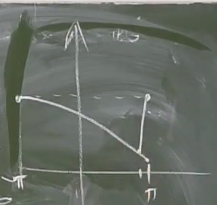
\includegraphics[scale=0.5]{img/periodic_to_C.png}
	\end{figure}

	Используя транзитивность свойства полноты, получим, что $\{e_k\}_{k = 1}^\infty$ -- полна в $L_p[-\pi,\,\pi]$, в частности в $L_{2\pi}^2$.
\end{proposition}

\begin{proposition}
	Посчитаем коэффициенты Фурье для нашей ортогональной системы в явном виде:

	Если $e_k = \cos(nx)$, то $f_k = \frac{\int_{-\pi}^\pi f(x)\cos(nx)d\mu(x)}{\int_{-\pi}^\pi \cos^2(nx)dx} = a_n$.
	Если $e_k = \sin(nx)$, то $f_k = b_n$.
	Ну и $e_1 = a_0$.
\end{proposition}

\begin{proposition}
	Равенство Парсеваля для тригонометрической системы в $L^2_{2\pi}$ будет иметь вид:
	\[\|f\|^2 = a_0^2\cdot\frac{\pi}{2} + \sum_{k = 1}^\infty (a_n^2 + b_n^2)\pi\]
\end{proposition}

\begin{proposition}
	Теорема Рисса-Фишера даёт следующее следствие: если $\frac{a_0^2}{2} + \sum_{n = 1}^\infty (a_n^2 + b_n^2)$ сходится, то коэффициенты $a_0,\, \{a_n,\,b_n\}_{n = 1}^\infty$ -- коэффициенты тригонометрического ряда Фурье функции из $L_{2\pi}^2$.
\end{proposition}

\section{Теорема Рисса-Фишера}
\begin{theorem}
	Рисса-Фишера.

	Если $\{e_k\}_{k = 1}^\infty$ -- ортогональная система ненулевых элементов гильбертова пространства $H$ и $\{\alpha_k\}_{k = 1}^\infty$ -- последовательность действительных чисел, такая что $\sum_{k = 1}^\infty \alpha_k^2 \|e_k\|^2$ сходится, то ряд $\sum_{k = 1}^\infty \alpha_ke_k$ сходится к некоторому $f \in H$.
\end{theorem}

\begin{proof}
	$\sum_{k = 1}^\infty \alpha_k^2\|e_k\|^2$ сходится $\stackrel{\text{к. Коши}}{\Rightarrow}$
	\[\forall \varepsilon > 0 \: \exists N \in \mathbb{N} \: \forall n > N,\, \forall p \in \mathbb{N}:\: \sum_{k = n + 1}^{n + p} \alpha_k^2\|e_k\|^2 < \varepsilon\]
	Тогда оценим норму некого элемента из $H$:
	\[\|\sum_{k = n + 1}^{n + p}\alpha_ke_k\|^2 = \langle\sum_{k = n + 1}^{n + p}\alpha_ke_k,\, \sum_{k = n + 1}^{n + p}\alpha_ke_k\rangle = \sum_{k = n + 1}^{n + p}\alpha_k^2\|e_k\|^2 < \varepsilon\]
	Это означает, что последовательность частичных сумм нашего ряда является фундаментальной, а значит благодаря гильбертовости пространства $H$ мы можем сказать, что ряд сходится.

	Что и требовалось доказать.
\end{proof}

\begin{corollary}
	Если $\{e_k\}_{k = 1}^\infty$ -- ортогональная система ненулевых элементов гильбертова пространства $H$, то $\forall f \in H\: \text{р. Фурье сходится к }f_0 \in H:\: \sum_{k = 1}^\infty f_ke_k = f_0$, то
	\[\langle f - f_0,\, e_j\rangle = 0,\, \forall j \in \mathbb{N}\]
\end{corollary}

\begin{proof}
	Из неравенства Бесселя следует:
	\[\sum_{k = 1}^\infty f_k^2\|e_k\|^2 < +\infty \stackrel{\text{т. Р-Ф}}{\Rightarrow} \exists f_0 \in H :\: \sum_{k = 1}^\infty f_ke_k = f_0 \Rightarrow \langle f - f_0,\,e_j\rangle = \langle f,\,e_j\rangle - f_j\|e_j\|^2 = 0\]
\end{proof}

\section{Полнота и замкнутость ортогональной системы, их связь}
\begin{definition}
	Система функций $\{\phi_n\}_{n = 1}^\infty$, называется полной в $L_p(E)$, если
	\[\forall \varepsilon > 0 \: \forall f \in L_p(E)\: \exists \{c_1,\,\cdots,\,c_n\} \subset \mathbb{R}:\: \|f - \sum_{k = 1}^n c_k\phi_k\|_p < \varepsilon\]
\end{definition}

\begin{definition}
	Система $\{e_k\}_{k = 1}^\infty$ называется замкнутой в евклидовом пространстве $E$ (по Банаху, в банаховом пространстве тотальной, в $C$ и $L_p$ -- полной), если 
	\[\forall k \in \mathbb{N}:\: \langle f,\, e_k\rangle = 0 \Rightarrow f = 0\]
\end{definition}

\begin{theorem}
	О связи.

	$\{e_k\}_{k = 1}^\infty$ -- замкнутая система в гильбертовом пространстве $\Leftrightarrow$ она полная.
\end{theorem}

\begin{proof}
	$\Rightarrow \{e_k\}_{k = 1}^\infty$ -- замкнутая $\stackrel{\text{сл-е т.Р-Ф}}{\Rightarrow} \forall f \in H:\: f = \sum_{k = 1}^\infty f_ke_k$
	Тогда, применяя следствие теоремы (\ref{THREE_EQUIV}) получим полноту системы.

	$\Leftarrow \{e_k\}_{k = 1}^\infty$ -- полная система, $\forall k \in \mathbb{N} \: \forall f \in H:\: \langle f,\,e_k\rangle = 0 \Rightarrow f_k = 0$. Теперь снова применим следствие теоремы (\ref{THREE_EQUIV}) и свойства полноты системы, получим, что $f = \sum 0e_k = 0$.
\end{proof}

\section{Полнота пространств $C[a,\,b]$ и $L_p[a,\,b],\, p > 1$}
\begin{definition}
	Для $1 < p < +\infty$ обозначим через $q$ такое число, что $\frac{1}{p} + \frac{1}{q} = 1$.
\end{definition}

\begin{lemma}
	$\forall a,\,b > 0 \: \forall p \in (1,\,+\infty):\: ab \leq \frac{a^p}{p} + \frac{b^q}{q}$
\end{lemma}
\begin{proof}
	Геометрическое:

	\begin{figure}[h] \caption{Геометрическое доказательство Л13.1}
		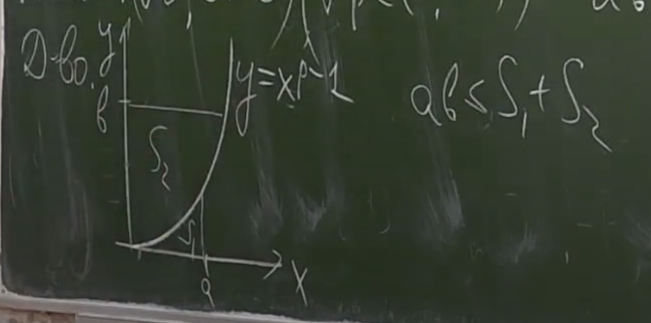
\includegraphics[scale=0.5]{img/yung.png}
	\end{figure}

	Причём $S_1$ и $S_2$ можно легко посчитать:
	\[S_1 = \int_0^a x^{p - 1}dx = \frac{a^p}{p}\;\;\;\; S_2 = \int_0^b y^{q - 1} = \frac{b^q}{q}dy\]
\end{proof}

\begin{theorem}
	Неравенство Гёльдера.

	Если $f \in L_p(X),\, g \in L_q(X),\, \frac{1}{p} + \frac{1}{q} = 1,\, 1 < p < +\infty$, то
	\[\int_X |f(x)g(x)|d\mu(x) \leq \left(\int_X |f(x)|^pd\mu(x)\right)^{\frac{1}{p}}\left(\int_X |g(x)|^qd\mu(x)\right)^{\frac{1}{q}}\]
\end{theorem}

\begin{proof}
	Если правая часть равна нулю, то всё доказано.

	Иначе введём обозначения:
	\[A^p := \int_X|f(x)|^pd\mu(x),\;\;\; B^q := \int_X|g(x)|^qd\mu(x)\]
	Тогда, используя предыдущую лемму с параметрами:
	\[a = \frac{|f(x)|}{A}\;\;\;\; b = \frac{|g(x)|}{B}\]
	Получим, что
	\[\frac{|f(x)||g(x)|}{AB} \leq \frac{|f(x)|^p}{pA^p} + \frac{|g(x)|^q}{qB^q}\]
	Теперь проинтегрируем обе части по $x$ и получим требуемое:
	\[\frac{\int_X |f(x)||g(x)|d\mu(x)}{AB} \leq \frac{1}{p} + \frac{1}{q} = 1\]
\end{proof}

\begin{theorem}
	Неравенство Минковского.

	Если $f,\, g \in L_p(E)$, то
	\[\left(\int_E |f(x) + g(x)|^p d\mu(x)\right)^{\frac{1}{p}} \leq \left(\int_E |f(x)|^p d\mu(x)\right)^{\frac{1}{p}} + \left(\int_E |g(x)|^p d\mu(x)\right)^{\frac{1}{p}}\]
\end{theorem}

\begin{proof}
	Очевидно, что $|f(x) + g(x)|^p \leq 2^p \max(|f(x)|^p,\, |g(x)|^p)$, поэтому $|f(x) + g(x)|^p$ будет суммируемая.

	Если $p = 1$, то всё очевидно -- неравенство треугольника, поэтому будем доказывать лишь для $1 < p < +\infty$.

	Распишем $|f(x) + g(x)|^p = |f(x) + g(x)|^{p - 1}|f(x) + g(x)|$. Теперь дважды применим неравенство Гёльдера, в первый раз $F(x) = f(x),\, G(x) = |f(x) + g(x)|^{p - 1}$. Во второй же -- $F(x) = g(x),\, G(x) = |f(x) + g(x)|^{p - 1}$. Получим, что:
	\begin{align*}
		\int_E |f(x) + g(x)|^p d\mu(x) \leq \\
		\left(\left(\int_E |f(x)|^pd\mu(x)\right)^{\frac{1}{p}} + \left(\int_E |g(x)|^pd\mu(x)\right)^{\frac{1}{p}}\right) \cdot \left(\int_E |f(x) + g(x)|^{(p - 1)q}d\mu(x)\right)^{\frac{1}{q}}
	\end{align*}
	Давайте более подробно распишем $(p - 1)q = (p - 1)\cdot\frac{1}{1 - \frac{1}{p}} = 0$, то есть второй множитель правой части неравенства под степенью имеет то же самое, что и левая часть, значит поделим обе части на неотрицательный $\left(\int_E |f(x) + g(x)|^{(p - 1)q}d\mu(x)\right)^{\frac{1}{q}}$ и получим:
	\[\left(\int_E |f(x) + g(x)|^p d\mu(x)\right)^{1 - \frac{1}{q} = \frac{1}{p}} \leq \left(\int_E |f(x)|^pd\mu(x)\right)^{\frac{1}{p}} + \left(\int_E |g(x)|^pd\mu(x)\right)^{\frac{1}{p}}\]
\end{proof}

\begin{corollary}
	Только теперь мы можем говорить, что $L_p(E)$ -- ЛНП с корректно определённой нормой (заметим, что неравенство Минковского -- это неравенство треугольника для этой нормы, остальные свойства очевидно следуют из свойств интеграла Лебега):
	\[\|f\|_p = \left(\int_E |f(x)|^p d\mu(x)\right)^{\frac{1}{p}}\]
\end{corollary}

\begin{theorem}
	Для $p \in [1,\,+\infty) \: L_p([a,\,b])$ -- банахово пространство.
\end{theorem}

\begin{proof}
	Пусть $\{f_n\}_{n = 1}^\infty$ -- фундаментальная последовательность в $L_p[a,\,b]$:
	\[\forall \varepsilon > 0 \: \exists N \in \mathbb{N} \: \forall n,\,m > N :\: \|f_n - f_m\|_p < \varepsilon\]
	Отсюда получаем, что $\exists \{n_k\}_{k = 1}^\infty \uparrow \: \forall m \geq n_k :\: \|f_m - f_{n_k}\|_p < \frac{1}{2^k}$.

	Тогда в силу неравенства Гёльдера:
	\[\|f_m - f_{n_k}\|_1 \leq \|f_m - f_{n_k}\|_p \cdot \|1\|_q < \frac{C}{2^k}\]

	Рассмотрим ряд
	\[\Phi(x) = |f_{n_1}(x)| + \sum_{k = 2}^\infty |f_{n_k}(x) - f_{n_{k-1}}(x)|\]
	И для него верно равенство (по теореме Леви):
	\[\|\Phi\|_1 = \|f_{n_1}\|_1 + \sum_{k = 2}^\infty \|f_{n_k} - f_{n_{k-1}}\|_1 < +\infty\]

	Значит $\Phi(x)$ конечная почти всюду $\Rightarrow$ ряд $|f_{n_1}(x)| + \sum_{k = 2}^\infty |f_{n_k}(x) - f_{n_{k-1}}(x)|$ -- сходится почти всюду на $[a,\,b]$.

	Тогда ряд $f_{n_1}(x) + \sum_{k = 2}^\infty (f_{n_k}(x) - f_{n_{k-1}}(x))$ сходится абсолютно почти всюду на $[a,\,b]$, но его частичные суммы -- это $f_{n_k} \Rightarrow$ мы получили, что эта последовательность сходится почти всюду к чему-то, что мы обозначим, как $f(x)$.

	Докажем, что $f \in L_p[a,\,b]$: если есть сходимость почти всюду, то по теореме Фату мы можем оценить:
	\[\int_{[a,\,b]}|f(x)|^pd\mu(x) \leq \underline{\lim\limits_{k \to +\infty}} \int_{[a,\,b]}|f_{n_k}(x)|^pd\mu(x) = \|f_{n_k}\|_p^p < +\infty\]
	Снова используем свойство последовательности $\{n_k\}_{k = 1}^\infty$:
	\[\forall \varepsilon > 0 \: \exists N \in \mathbb{N} \: \forall k,\,l > N :\: \|f_{n_k} - f_{n_l}\|_p < \varepsilon\]
	Но мы можем перейти к пределу $l \to +\infty$ благодаря теореме Лебега: $\|f_{n_k} - f\|_p < \varepsilon$. Тогда при достаточно больших $m$:
	\[\|f_m - f\|_p \leq \|f_m - f_{n_k}\|_p + \|f_{n_k} - f\|_p < 2\varepsilon\]
\end{proof}

\begin{theorem}
	$C[a,\,b]$ -- полно
\end{theorem}

\begin{proof}
	Рассмотрим для определённости $\rho(f,\,g) = \sup_{x \in [a,\,b]}|f(x) - g(x)|$.

	Пусть последовательность $\{f_n(x)\}_{n = 1}^\infty$ -- фундаментальна. Зафиксируем $x_0 \in [a,\,b]$.

	Тогда $\{f_n(x_0)\}_{n = 1}^\infty$ фундаментальная числовая последовательность $\Rightarrow$ она сходится. Обозначим этот предел как $f(x_0)$.

	Очевидно, $f_n(x) \stackrel{n \to +\infty}{\to} f(x)$ по введённой метрике, так как:
	\[\forall \varepsilon > 0 \: \exists N_\varepsilon \: \forall n,\,m \geq N_\varepsilon \: \forall x \in [a,\,b] :\: |f_n(x) - f_m(x)| < \varepsilon\]
	Зафиксируем $x$ и перейдём к пределу при $m \to +\infty \Rightarrow$ при всех тех же кванторах выполняется неравенство $|f_n(x) - f(x)| \leq \varepsilon$. Значит $f_n(x) \rightrightarrows f(x)$, тогда по теореме о равномерном пределе непрерывных функций $f(x) \in C[a,\,b]$. Что и требовалось доказать.
\end{proof}

\section{Непрерывность, интегрируемость и дифференцируемость интегралов, зависящих от параметра}
\begin{definition}
	Пусть функция $f(x,\,\alpha)$ зависит от $x,\, \alpha$. Тогда мы можем рассматривать функцию $f_{1,\,\alpha}(x)$ -- изначальная функция, которую мы теперь считаем зависящей только от первого параметра, а второй параметр считаем фиксированным. Аналогично вводится $f_{2,\,x}(\alpha)$.
\end{definition}

\begin{theorem}
	Непрерывность интеграла, зависящего от параметра

	Пусть $\forall \alpha \in A \subset \mathbb{R}^n$ функция $f_{1,\,\alpha}(x) = f(x,\,\alpha)$ суммируема на $E \subset \mathbb{R}^m$, $f_{2,\,x}(\alpha) = f(x,\,\alpha)$ при почти всех $x \in E$ непрерывна в $\alpha_0 \in E$, и при почти всех $x \in E,\, \forall \alpha \in A :\: |f(x,\,\alpha)| \leq \phi(x)$, где $\phi(x)$ суммируема на $E$. Тогда
	\[F(\alpha) = \int_E f(x,\, \alpha)d\mu(x)\]
	непрерывна в $\alpha_0$.
\end{theorem}

\begin{proof}
	Рассмотрим $\forall \{\alpha_n\}_{n = 1}^\infty \subset A,\, \lim\limits_{n\to +\infty}\alpha_n = \alpha_0$.

	Тогда, по условию, $\lim\limits_{n \to +\infty} f(x,\,\alpha_n) = f(x,\,\alpha_0)$ при почти всех $x \in E$. Кроме того, для почти всех $x$ из $E$, выполняется неравенство $\forall n \in \mathbb{N}:\: |f(x,\,\alpha_n)| \leq \phi(x)$. Тогда, используя теорему Лебега, мы сможем перейти к пределу интегралов:
	\[F(\alpha_n) = \int_E f_{1,\, \alpha_n}(x)d\mu(x) \stackrel{n \to +\infty}{\to} \int_E f(x,\,\alpha_0)d\mu(x) = F(\alpha_0)\]
\end{proof}

\begin{theorem}
	Дифференцируемость интеграла, зависящего от параметра

	Пусть $f_{1,\,\alpha}(x) = f(x,\,\alpha)$ при всех $\alpha \in U(\alpha_0) \subset \mathbb{R}^n$ суммируема на $E \subset \mathbb{R}^m$ вместе с $\frac{\partial f(x,\,\alpha)}{\partial \alpha}$, и при почти всех $x \in E,\, \forall \alpha \in U(\alpha_0)$: $\left|\frac{\partial f(x,\,\alpha)}{\partial \alpha}\right| \leq \phi(x)$, где $\phi(x)$ суммируема на $E$. Тогда
	\[F'(\alpha_0) = \int_E \frac{\partial f(x,\,\alpha_0)}{\partial \alpha}d\mu(x)\]
\end{theorem}

\begin{proof}
	Рассмотрим $\forall \{\alpha_n\}_{n = 1}^\infty \subset \dot{U}(\alpha_0),\, \lim\limits_{n \to +\infty}\alpha_n = \alpha_0$.

	Тогда частная производная в точке $\alpha_0$ -- это
	\[\left|\frac{f(x,\,\alpha_n) - f(x,\,\alpha_0)}{\alpha_n - \alpha_0}\right| = \left|\frac{\partial f(x,\,\xi_n(x))}{\partial \alpha}\right| \leq \phi(x)\]
	Теперь, используя теорему Лебега, получим равенство пределов интегралов:
	\[\lim_{n \to +\infty}\int_E \frac{f(x,\,\alpha_n) - f(x,\,\alpha_0)}{\alpha_n - \alpha_0}d\mu(x) = \int_E \frac{\partial f(x,\,\alpha_0)}{\partial	\alpha}d\mu(x)\]
\end{proof}

\section{Равномерная сходимость несобственных интегралов, зависящих от параметра. Критерий Коши, признаки Вейерштрасса и Дирихле}
\begin{definition}
	Пусть $f(x,\,y) \in \mathcal{R}[a,\,\tilde{b}] \: \forall \tilde{b} < b \: \forall y \in A \subset \mathbb{R}$. Тогда несобственным интегралом Римана, зависящим от параметра $y$ называется
	\begin{equation} \label{NESOBS_INT}
		\int_a^b f(x,\,y)dx = \lim_{\tilde{b} \to b - 0} \int_a^{\tilde{b}}f(x,\,y)dx
	\end{equation}
\end{definition}

\begin{definition}
	Мы говорим, что несобственный интеграл (\ref{NESOBS_INT}) сходится поточечно, если:
	\[\forall y \in A \: \forall \varepsilon > 0 \: \exists B \in (a,\,b) \: \forall B' \in (B,\,b):\: \left|\int_{B'}^b f(x,\,y)dx\right| < \varepsilon\]
\end{definition}

\begin{definition}
	Несобственный интеграл (\ref{NESOBS_INT}) сходится равномерно на $A$, если:
	\[\forall \varepsilon > 0 \: \exists B \in (a,\,b) \: \forall B' \in (B,\,b) \: \forall y \in A :\: \left|\int_{B'}^b f(x,\,y)dx\right| < \varepsilon\]
\end{definition}

\begin{theorem}
	Критерий Коши равномерной сходимости интегралов, зависящих от параметра

	(\ref{NESOBS_INT}) сходится равномерно на $A \Leftrightarrow$
	\[\forall \varepsilon > 0 \: \exists B \in (a,\,b) \: \forall a < B' < B''< b \: \forall y \in A :\: \left|\int_{B'}^{B''}f(x,\,y)dx\right| < \varepsilon\]
\end{theorem}

\begin{proof}
	$\Rightarrow$ При всех требуемых кванторах можем сделать оценку:
	\[\left|\int_{B'}^{B''}f(x,\,y)dx\right| = \left|\int_{B''}^b f(x,\,y)dx - \int_{B'}^bf(x,\,y)dx\right| < 2\varepsilon\]
	$\Leftarrow$ Фиксируем $\forall y \in A$, тогда используем критерий Коши сходимости несобственных интегралов (без параметра), то есть
	\[\int_a^b f(x,\,y)dx < +\infty \stackrel{B'' \to b - 0}{\Rightarrow} \left|\int_{B'}^{b}f(x,\,y)dx\right| \leq \varepsilon\]
\end{proof}

\begin{corollary}
	Признак сравнения.

	Если $|f(x,\,y)| < g(x,\,y)$, $f,\,g$ удовлетворяют условиям определения несобственных интегралов Римана, $\int_a^b g(x,\,y)dx$ равномерно сходится на $A$, то $\int_a^b f(x,\,y)dx$ равномерно сходится на $A$.
\end{corollary}

\begin{corollary}
	Признак Вейерштрасса.

	Если $|f(x,\,y)| \leq g(x)$, $f,\,g$ удовлетворяют условиям определения несобственных интегралов Римана, $\int_a^b g(x)dx$ сходится на $A$, то $\int_a^b f(x,\,y)dx$ равномерно сходится на $A$.
\end{corollary}

\begin{theorem}
	Признак Дирихле равномерной сходимости НИРЗП.

	\begin{enumerate}
		\item $f \in \mathcal{R}[a,\,\tilde{b}]\:\forall \tilde{b} \in (a,\,b) \: \forall y \in A$ и $\forall y \in A$:
		      \[\left|\int_a^x f(t,\,y)dt\right| \leq C\]
		\item $g(x,\,y) \downarrow 0$ при $x \to b - 0$ равномерно по $y \in A$.
	\end{enumerate}
	Тогда $\int_a^b f(x,\,y)g(x,\,y)dx$ равномерно сходится на $A$.
\end{theorem}
\begin{proof}
	По формуле Бонне:
	\[\int_{B'}^{B''}f(x,\,y)g(x,\,y)dx = g(B',\,y)\int_{B'}^{\xi(y)}f(x,\,y)dx + g(B'',\,y)\int_{\xi(y)}^{B''}f(x,\,y)dx\]
	$g \rightrightarrows 0$, значит
	\[\forall \varepsilon > 0 \: \exists B \in (a,\,b) \: \forall x \in (B,\,b) \: \forall y \in A :\: |g(x,\,y)| < \frac{\varepsilon}{4C}\]
	А все интегралы в полученной формуле можно оценить сверху, как $2C$, поэтому получим, что
	\[\left|\int_{B'}^{B''}f(x,\,y)g(x,\,y)dx\right| \leq \frac{\varepsilon}{4C}\cdot 2C + \frac{\varepsilon}{4C}\cdot 2C = \varepsilon\]
\end{proof}

\section{Непрерывность и интегрируемость несобственных интегралов, зависящих от параметра}
\begin{theorem}
	Непрерывность НИРЗП

	Если $f(x,\,y)$ непрерывна на $[a,\,b) \times [c,\,d]\; (b \leq +\infty)$ и $\int_a^bf(x,\,y)dx$ равномерно сходится на $[c,\,d]$, то он является непрерывной функцией на $[c,\,d]$.
\end{theorem}
\begin{proof}
	Рассмотрим произвольную $\{b_n\}_{n = 1}^\infty \subset [a,\,b],\,\lim\limits_{n \to +\infty}b_n = b$, а также введём
	\[I_n(y) := \int_a^{b_n}f(x,\,y)dx\]
	Равномерная сходимость $\int_a^bf(x,\,y)dx$ влечёт равномерную сходимость $I_n(y)$. Используя теорему о пределе равномерно сходящейся функциональной последовательности получим, что $\lim\limits_{n \to +\infty} I_n(y)$ -- непрерывная.
\end{proof}

\begin{theorem}
	Собственная интегрируемость НИРЗП.

	Если $f(x,\,y)$ непрерывна на $[a,\,b) \times [c,\,d]\;(b \leq +\infty)$ и $\int_a^b f(x,\,y)dx$ равномерно сходится на $[c,\,d]$, то
	\[\int_a^b \left(\int_c^d f(x,\,y)dy\right)dx = \int_c^d\left(\int_a^b f(x,\,y)dx\right)dy\]
\end{theorem}
\begin{proof}
	Рассмотрим произвольную последовательность $\{b_n\}_{n = 1}^\infty \subset [a,\,b),\, \lim\limits_{n\to +\infty} b_n = b$. Положим
	\[I_n(y) := \int_a^{b_n}f(x,\,y)dx\]
	Тогда равномерная сходимость $\int_a^b f(x,\,y)dx$ влечёт равномерную сходимость $I_n(y)$.

	Используя прыдыдущую теорему и теорему об интегрируемости функциональных последовательностей и тот факт, что $f(x,\,y)$ непрерывна на прямоугольнике $[a,\,b_n]\times [c,\,d]$, поэтому мы можем переставить пределы интегрирования и получим:
	\[\int_a^{b_n}\left(\int_c^d f(x,\,y)dy\right)dx = \int_c^d I_n(y)dy \stackrel{n \to +\infty}{\to} \int_c^d \left(\int_a^b f(x,\,y)dx\right)dy\]
\end{proof}

\section{Дифференцирование несобственных интегралов по параметру}
\begin{theorem}
	Дифференцируемость НИРЗП.

	Если $f(x,\,y)$ и $\frac{\partial f}{\partial y}(x,\,y)$ непрерывны на $[a,\,b) \times [c,\,d],\, \int_a^b \frac{\partial f}{\partial y}(x,\,y)dx$ сходится равномерно на $[c,\,d]$, $\int_a^b f(x,\,y)dx$ сходится для некоторого $y_0 \in [c,\,d]$, то $I(y) = \int_a^b f(x,\,y)dx$ сходится и является дифференцируемой функцией на $[c,\,d]$, причём
	\[I'(y) = \int_a^b \frac{\partial f}{\partial y}(x,\,y)dx\]
\end{theorem}
\begin{proof}
	$\forall t \in [c,\,d]$ и фиксированного $x \in [a,\,b]$ справедлива формула
	\[f(x,\,t) = f(x,\,y_0) + \int_{y_0}^t \frac{\partial f}{\partial y}(x,\,y)dy\]
	Тогда, если мы проинтегрируем обе части по $[a,\,b]$ по $x$, то получим что
	\begin{enumerate}
		\item Первое слагаемое сходится по условию
		\item Второе слагаемое удовлетворяет условию теоремы о собственной интегрируемости несобственного интеграла, а это значит что он сходится по $x$.
	\end{enumerate}
	Значит и интеграл от левой части также сходится $\forall t$, причём он равен
	\[I(t) := \int_a^b f(x,\,y_0)dx + \int_a^b \left(\int_{y_0}^t \frac{\partial f}{\partial y}(x,\,y)dy\right)dx = \int_a^b f(x,\,y_0)dx + \int_{y_0}^t \left(\int_a^b \frac{\partial f}{\partial y}(x,\,y) dx\right)dy\]
	Тогда при взятии производной $I'(t)$, первое слагаемое обнулится, а второе, являясь переменным верхним пределом, превратится в $\int_a^b \frac{\partial f}{\partial y}(x,\,t) dx$.
\end{proof}

\section{Гамма- и бета-функции и связь между ними}
\begin{definition}
	Гамма-функцией называется
	\[\Gamma(\alpha) := \int_0^{+\infty}x^{\alpha - 1}e^{-x}dx,\; \alpha > 0\]
\end{definition}

\begin{proposition}
	Гамма-функция сходится
\end{proposition}

\begin{proof}
	\[\Gamma(\alpha) = \int_0^1 x^{\alpha - 1}e^{-x}dx + \int_1^{+\infty} x^{\alpha - 1}e^{-x}dx =: I_1(\alpha) + I_2(\alpha)\]
	$I_1$ сходится по признаку сравнения, так как
	\[x^{\alpha - 1}e^{-x} \leq x^{\alpha - 1},\;\;\; \int_0^1 x^{\alpha - 1}dx < +\infty,\, \alpha > 0\]
	$I_2$ также сходится по признаку сравнения, так как
	\[x^{\alpha - 1}e^{-x} \leq Ce^{-\frac{x}{2}},\, x \geq 1 ;\;\; \int_1^{+\infty} e^{-\frac{x}{2}}dx < +\infty\]
\end{proof}

\begin{theorem}
	Основные свойства гамма-функции.

	\begin{enumerate}
		\item $\Gamma(\alpha)$ бесконечно дифференцируема $\forall \alpha > 0$.
		\item Формула понижения. $\Gamma(\alpha + 1) = \alpha\Gamma(\alpha),\, \alpha > 0$
		\item $\Gamma(n + 1) = n!\;\;\; n \in \mathbb{N} \cup \{0\}$
	\end{enumerate}
\end{theorem}
\begin{proof}
	\begin{enumerate}
		\item $(x^{\alpha - 1}e^{-x})'_\alpha = x^{\alpha - 1}e^{-x}\ln x$, заметим, что все оценки, сделанные в предыдущем пункте сохранятся (с немного изменённым коэффициентом $\alpha$), так как
		      \[\ln x \leq \frac{1}{x^\varepsilon},\,x\in(0,\,1];\;\;\; \ln x \leq x^\varepsilon,\, x \geq 1\]
		      Значит мы можем дифференцировать сколько угодно раз с сохранением сходимости.
		\item Проинтегрировав по частям, получим:
		      \[\Gamma(\alpha + 1) = -x^\alpha e^{-x}|^{+\infty}_0 + \alpha\int_0^{+\infty}x^{\alpha - 1}e^{-x}dx = \alpha\Gamma(\alpha)\]
		\item Заметим, что $\Gamma(1) = \int_1^{+\infty} e^{-x}dx = -e^{-x}|^{+\infty}_0 = 1$. Используя предыдущее свойство, доказываемое утверждение становится очевидным.
	\end{enumerate}
\end{proof}

\begin{definition}
	Бета-функцией называется $B(a,\,b) = \int_0^1 x^{a - 1}(1 - x)^{b - 1}dx;\; a,\,b \geq 0$
\end{definition}

\begin{theorem}
	Связь бета- и гамма-функций.

	$\forall a,\,b > 0:\: B(a,\,b) = \frac{\Gamma(a)\Gamma(b)}{\Gamma(a + b)}$
\end{theorem}

\begin{proof}
	\[
		B(a,\,b)\Gamma(a + b) = \int_0^1 x^{a - 1}(1 - x)^{b - 1}dx\int_0^{+\infty} y^{a + b - 1}e^{-y}dy \stackrel{?}{=} \int_0^{+\infty}\xi^{a - 1}e^{-\xi}d\xi \int_0^{+\infty}\eta^{b - 1}e^{-\eta}d\eta
	\]
	Будем рассматривать оба интеграла, как двойные. Рассмотрим замену координат вида
	\[
		\begin{cases}
			xy = \xi \\
			(1 - x)y = \eta
		\end{cases}
		\Rightarrow
		\begin{cases}
			y = \xi + \eta \\
			x = \frac{\xi}{\xi + \eta}
		\end{cases}
		\Rightarrow
		\frac{\partial(\xi,\,\eta)}{\partial(x,\,y)} =
		\begin{vmatrix}
			y  & x     \\
			-y & 1 - x
		\end{vmatrix}
		= y(1 - x + x) = y \neq 0
	\]
	Проведите данную замену и у вас всё обязательно получится!
\end{proof}

\section{Формула Гаусса-Эйлера для гамма-функции}
\begin{theorem}
	Формула Гаусса-Эйлера.

	Для любых $\alpha > 0$:
	\[\Gamma(\alpha) = \lim_{n \to +\infty}n^\alpha \frac{(n - 1)!}{\alpha(\alpha + 1)\cdots (\alpha + n - 1)}\]
\end{theorem}
\begin{proof}
	Напоминаем, что
	\[
		\Gamma(\alpha) = \int_0^{+\infty}x^{\alpha - 1}e^{-x}dx \stackrel{e^{-x} =: u}{=} \int_0^1 \ln^{\alpha - 1}\frac{1}{u}du
	\]
	Докажем, что $f_n(u) = n(1 - u^{\frac{1}{n}})$ монотонно стремится к $\ln\frac{1}{u},\, u \in (0,\,1]$. Для этого рассмотрим функцию $g(t,\,u) = t(1 - u^{\frac{1}{t}})$. Тогда
	\[\frac{\partial g}{\partial t} = 1 - u^{\frac{1}{t}} - t\cdot u^{\frac{1}{t}}\ln u\cdot (-\frac{1}{t^2}) = 1 - u^{\frac{1}{t}} + u^{\frac{1}{t}}\ln u^{\frac{1}{t}},\, u \in (0,\,1],\, t > 0\]
	Обозначив $y := u^{\frac{1}{t}} \Rightarrow y \in (0,\,1]$ получим новую функцию $\phi(y) = 1 - y + y\ln y$. Тогда
	\[\phi'(y) = -1 + \ln y + 1 = \ln y < 0,\, y \in (0,\,1];\;\;\; \phi(1) = 0 \Rightarrow \phi(y) \geq 0 \Rightarrow g \geq 0 \Rightarrow f_n(u) \uparrow\]
	Тогда рассмотрим предел
	\[\lim_{n \to +\infty} f_n(u) = \lim_{n \to +\infty} \frac{1 - e^{\frac{1}{n}\ln u}}{\frac{1}{n}} \stackrel{\text{2й зам-й пр-л}}{=} \lim_{n \to +\infty}\frac{-\frac{1}{n}\ln u}{\frac{1}{n}} = -\ln u = \ln\frac{1}{u}\]
	Значит мы можем применить теорему Леви для последовательности $f_n(u)$:
	\[\int_0^1 (n(1 - u^{\frac{1}{n}}))^{\alpha - 1}du \stackrel{n \to +\infty}{\to} \int_0^1 \ln^{\alpha - 1}\frac{1}{u}du\]
	То есть мы получили, что
	\begin{align*}
		\Gamma(\alpha) = \lim_{n \to +\infty} n^{\alpha - 1}\int_0^1 (1 - u^{\frac{1}{n}})^{\alpha - 1}du \stackrel{u = t^n}{=} \lim_{n \to +\infty}n^\alpha \int_0^1 t^{n - 1}(1 - t)^{\alpha - 1}dt = \lim_{n \to +\infty} n^\alpha B(n,\,\alpha) = \\
		\lim_{n \to +\infty} n^\alpha \frac{\Gamma(n)\Gamma(\alpha)}{\Gamma(\alpha + n)} = \lim_{n \to +\infty}n^\alpha \frac{(n - 1)!\Gamma(\alpha)}{(\alpha + n - 1)\cdots\alpha\Gamma(\alpha)} = \lim_{n \to +\infty}n^\alpha \frac{(n - 1)!}{\alpha(\alpha + 1)\cdots (\alpha + n - 1)}
	\end{align*}
\end{proof}

\section{Формула Валлиса. Представление синуса в виде бесконечного произведения.}
\begin{theorem}
	Формула Валлиса.

	Для любого $\alpha \in \mathbb{R},\, |\alpha| < 1$:
	\[\frac{\sin \alpha\pi}{\alpha\pi} = \prod_{n = 1}^\infty \left(1 - \frac{\alpha^2}{n^2}\right)\]
\end{theorem}
\begin{proof}
	Рассмотрим функцию $\cos\alpha x$ на $[-\pi,\,\pi]$, разложим её в тригонометрический ряд Фурье:
	\begin{align*}
		b_n = 0,\, a_n = \frac{2}{\pi}\int_0^\pi\cos\alpha x\cos nxdx = \frac{1}{\pi}\int_0^\pi(\cos(\alpha + n)x + \cos(\alpha - n)x)dx =                                                                        \\
		\frac{1}{\pi}\left(\frac{\sin(\alpha + n)x}{\alpha + n} + \frac{\sin(\alpha - n)x}{\alpha - n}\right)|_0^\pi = \frac{(-1)^n\sin\alpha\pi}{\pi}\left(\frac{1}{\alpha + n} + \frac{1}{\alpha - n }\right) = \\
		\frac{2(-1)^n\alpha\sin\alpha\pi}{\pi(\alpha^2 - n^2)},\, n = 0,\,1,\,\cdots
	\end{align*}
	Значит
	\[\cos\alpha x = \frac{\sin\alpha\pi}{\alpha\pi} + \frac{2\alpha\sin\alpha\pi}{\pi}\sum_{n = 1}^\infty \frac{(-1)^n}{\alpha^2 - n^2}\cos nx,\, \alpha x \in [-\pi,\,\pi]\]
	Возьмём $x := \pi$, тогда
	\[\cos\alpha\pi = \frac{\sin\alpha\pi}{\alpha\pi}\left(1 + 2\frac{\alpha}{\pi}\sum_{n = 1}^\infty \frac{1}{\alpha^2 - n^2}\right) \Rightarrow \ctg\alpha\pi = \frac{1}{\alpha\pi} + 2\frac{\alpha}{\pi}\sum_{n=1}^\infty\frac{1}{\alpha^2 - n^2},\, |\alpha| < 1,\, \alpha \neq 0\]
	В итоге получим, что
	\[\ctg\alpha\pi  - \frac{1}{\alpha\pi} = 2\frac{\alpha}{\pi}\sum_{n=1}^\infty\frac{1}{\alpha^2 - n^2},\, |\alpha| < 1,\, \alpha \neq 0\]
	Где слева -- устранимая точка разрыва, а справа ряд равномерно сходится при $\alpha \leq \alpha_0 < 1$ (Можем оценить $\left|\frac{\alpha}{\alpha^2 - n^2}\right|\leq \frac{1}{n^2 - \alpha_0^2}$). Значит мы можем проинтегрировать обе части по $\alpha$:
	\begin{align*}
		\int_0^x \left(\ctg\alpha\pi  - \frac{1}{\alpha\pi}\right)d\alpha = \frac{2}{\pi}\sum_{n = 1}^\infty \int_0^x \frac{\alpha d\alpha}{\alpha^2 - n^2},\, |x| < 1 \Rightarrow           \\
		\left[\frac{1}{\pi}\ln|\sin\alpha\pi| - \frac{1}{\pi}\ln|\alpha|\right]|_0^x = \frac{1}{\pi}\sum_{n = 1}^\infty\ln|\alpha^2 - n^2||_0^x \Rightarrow                                  \\
		\frac{1}{\pi}\ln\frac{\sin\pi x}{x} - \frac{1}{\pi}\ln\frac{\sin\alpha\pi}{\alpha}|_{\alpha = 0} = \frac{1}{\pi}\sum_{n = 1}^\infty\left(\ln|x^2 - n^2| - \ln n^2\right) \Rightarrow \\
		\ln\frac{\sin\pi x}{\pi x} = \sum_{n = 1}^\infty \ln\left(1 - \frac{x^2}{n^2}\right)
	\end{align*}
\end{proof}

\section{Формула дополнения для гамма-функции}
\begin{theorem}
	Формула дополнения.

	Для любых $\alpha \in (0,\,1)$:
	\[\Gamma(\alpha)\Gamma(1 - \alpha) = \frac{\pi}{\sin\alpha\pi}\]
\end{theorem}
\begin{proof}
	Используем формулу Гаусса-Эйлера:
	\begin{align*}
		\Gamma(\alpha)\Gamma(1 - \alpha) = \lim_{n \to +\infty} n^\alpha\frac{(n - 1)!}{\alpha(\alpha + 1)\cdots(\alpha + n - 1)}\cdot n^{1 - \alpha}\frac{(n - 1)!}{(1 - \alpha)(2 - \alpha)\cdots(n - \alpha)} =                                                           \\
		\lim_{n \to +\infty}\frac{n((n - 1)!)^2(\alpha + n)}{\alpha(1 - \alpha^2)(2^2 - \alpha^2)\cdots(n^2 - \alpha^2)} = \lim_{n \to +\infty}\frac{\alpha + n}{\alpha}\cdot\frac{1}{n(1 - \frac{\alpha^2}{1})(1 - \frac{\alpha^2}{2^2})\cdots(1 - \frac{\alpha^2}{n^2})} = \\
		\frac{1}{\alpha\prod_{n = 1}^\infty\left(1 - \frac{\alpha^2}{n^2}\right)}\stackrel{\text{ф. Валлиса}}{=} \frac{1}{\alpha\frac{\sin\alpha\pi}{\alpha\pi}} = \frac{\pi}{\sin\alpha\pi}
	\end{align*}
\end{proof}

\section{Равносходимость интеграла и ряда Фурье в точке}
\begin{definition}
	Пусть $f$ суммируема на $\mathbb{R}$. Интегралом Фурье функции $f$ называется
	\[I_f(x) = \int_0^{+\infty}(a(\lambda)\cos(\lambda x) + b(\lambda)\sin(\lambda x))d\lambda\]
	где
	\[a(\lambda) = \frac{1}{\pi}\int_\mathbb{R}f(t)\cos(\lambda t)d\mu(t);\;\;\; b(\lambda) = \frac{1}{\pi}\int_\mathbb{R} f(t)\sin(\lambda t)d\mu(t)\]
\end{definition}

\begin{theorem}
	Признак Дини сходимости интегралов Фурье.

	Пусть $f \in L_1(\mathbb{R})$, и для некоторого $x_0 \in \mathbb{R}\: \exists \delta > 0$ и $S(x_0)$, такие что
	\[\phi_{x_0}(t) := \frac{f(x_0 + t) + f(x_0 - t) - 2S(x_0)}{t} \in L_1(0,\,\delta)\]
	Тогда $I_f(x_0) = S(x_0)$
\end{theorem}
\begin{proof} \label{DINI_FURRY}
	Давайте распишем разность
	\begin{align*}
		I_f(x_0) - S(x_0) = \frac{1}{\pi}\int_0^{+\infty}\left[\int_\mathbb{R}f(t)\cos(\lambda (x_0 - t))d\mu(t)\right]d\lambda - S(x_0) \stackrel{u := x_0 - t}{=}              \\
		\frac{1}{\pi}\int_0^{+\infty}\left[\int_\mathbb{R}f(x_0 - u)\cos(\lambda u)d\mu(u)\right]d\lambda - S(x_0) =                                                             \\
		\frac{1}{\pi}\int_0^{+\infty}\left[\int_{[0,\,+\infty)}f(x_0 + u)\cos(\lambda u)d\mu(u) + \int_{[0,\,+\infty)}f(x_0 - u)\cos(\lambda u)d\mu(u)\right]d\lambda - S(x_0) = \\
		\frac{1}{\pi}\lim_{\Lambda \to +\infty}\int_0^\Lambda\int_{[0,\,+\infty)}(f(x_0 + u) + f(x_0 - u))\cos(\lambda u)d\mu(u)d\lambda - S(x_0)
	\end{align*}
	Мы можем сделать оценку
	\[|(f(x_0 + u) + f(x_0 - u))\cos(\lambda u)| \leq |f(x_0 + u) + f(x_0 - u)| \in L_1(\mathbb{R} \times [0,\, \Lambda])\]
	Значит мы можем применить теорему Фубини и переставить интегралы:
	\begin{align*}
		I_f(x_0) - S(x_0) = \frac{1}{\pi}\lim_{\Lambda \to +\infty} \int_{[0,\,+\infty)} (f(x_0 + u) + f(x_0 - u)) \int_0^\Lambda \cos(\lambda u)d\lambda d\mu(u) - S(x_0) = \\
		\frac{1}{\pi}\lim_{\Lambda \to +\infty} \int_{[0,\,+\infty)} (f(x_0 + u) + f(x_0 - u)) \frac{\sin(\Lambda u)}{u}d\mu(u) - S(x_0) =                                   \\
		\frac{1}{\pi}\left[\lim_{\Lambda \to +\infty} \int_{[0,\,+\infty)} (f(x_0 + u) + f(x_0 - u))\frac{\sin(\Lambda u)}{u}d\mu(u) - 2S(x_0)\int_{[0,\,+\infty)} \frac{\sin(\Lambda u)}{u}du\right]
	\end{align*}
	Последний переход получился из того факта (интеграл Дирихле), что
	\[\int_{[0,\,+\infty)}\frac{\sin(\Lambda u)}{u}du = \frac{\pi}{2},\, \Lambda > 0\]
	Продолжим расписывать\dots
	\begin{align*}
		I_f(x_0) - S(x_0) =                                                                                             \\
		\frac{1}{\pi}\lim_{\Lambda \to +\infty}\Big[\int_0^\delta\frac{f(x_0 + u) + f(x_0 - u) - 2S(x_0)}{u}\sin(\Lambda u)d\mu(u) + \\
			\int_{\delta}^{+\infty} \frac{f(x_0 + u) + f(x_0 - u)}{u}\sin(\Lambda u)d\mu(u) - 2S(x_0)\int_\delta^{+\infty}\frac{\sin(\Lambda u)}{u}du\Big]
	\end{align*}
	Рассмотрим каждое из этих слагаемых поотдельности:
	\begin{enumerate}
		\item По теореме Римана об осцилляции:
		      \[\int_{[0,\,\delta]}\phi_{x_0}(u)\sin(\Lambda u)d\mu(u) \stackrel{\Lambda \to +\infty}{\to} 0\]
		\item На $[\delta,\, +\infty)$ мы можем использовать следующую оценку:
		      \[\left|\frac{f(x_0 + u)}{u}\right| \leq \frac{1}{\delta}|f(x_0 + u)|\]
		      Значит по теореме Римана об осцилляции (предыдущим неравенством мы доказали, что $\frac{f(x_0 + u)}{u}$ суммируемая, аналогично для второго подслагаемого):
		      \[\int_{[\delta,\, +\infty)} \frac{f(x_0 + u)}{u}sin(\Lambda u) d\mu(u) \stackrel{\Lambda \to +\infty}{\to} 0\]
		\item Совершим замену и получим хвост сходящегося интеграла Римана (интеграла Дирихле):
		      \[\int_\delta^{+\infty}\frac{\sin(\Lambda u)}{u}du = \int_{\Lambda\delta}^{+\infty}\frac{\sin t}{t}dt \stackrel{\Lambda \to +\infty}{\to} 0\]
	\end{enumerate}
	Таким образом, теорема доказана.
\end{proof}

\begin{corollary}
	Если $f \in L_1(\mathbb{R})$ и удовлетворяет условию Гёльдера (\ref{GELDER}) порядка $\alpha,\, 0 < \alpha \leq 1$ в точке $x_0$, то $I_f(x_0) = \frac{f(x_0 + 0) + f(x_0 - 0)}{2}$.

	Если $f \in L_1(\mathbb{R}) \cap C^1(\mathbb{R})$, то $I_f(x) = f(x) ;\;\forall x \in \mathbb{R}$.
\end{corollary}

\section{Преобразование Фурье. Обратное преобразование Фурье. Свойства преобразования Фурье суммируемой функции. Формулы обращения.}
\begin{definition}
	Преобразованием Фурье функции $f$, суммируемой на $\mathbb{R}$ называется
	\[F[f] := \hat{f}(\lambda) = \frac{1}{\sqrt{2\pi}}\int_\mathbb{R}f(t)e^{-i\lambda t}d\mu(t)\]
\end{definition}

\begin{definition}
	Обратным преобразованием Фурье функции $F \in C(\mathbb{R})$ называется
	\[F^{-1}[f] := \tilde{F}(x) = \frac{1}{\sqrt{2\pi}} \text{v.p. }\int_{-\infty}^{+\infty}e^{i\lambda x}F(\lambda)d\lambda\]
\end{definition}

\begin{theorem}
	Свойства преобразования Фурье суммируемых на всей числовой оси функций.

	\begin{enumerate}
		\item (Линейность)

		      Если $f,\,g \in L_1(\mathbb{R}),\, \alpha,\, \beta \in \mathbb{R}$, то
		      \[\widehat{\alpha f + \beta g}(\lambda) = \alpha\hat{f}(\lambda) + \beta\hat{g}(\lambda)\]
		\item Если $f \in L_1(\mathbb{R})$, то $\hat{f}(\lambda)$ непрерывна на $\mathbb{R}$ и $\lim\limits_{\lambda \to \infty}\hat{f}(\lambda) = 0$.
		\item Если $f \in L_1(\mathbb{R}),\, \phi(x) = f(\alpha x),\, \alpha > 0$, то $\hat{\phi}(\lambda) = \frac{1}{\alpha}\hat{f}(\frac{\lambda}{\alpha})$
		\item Если $f \in L_1(\mathbb{R}),\, \psi(\lambda) = f(\lambda + a),\, a \in \mathbb{R}$, то $\hat{\psi}(\lambda) = e^{ia\lambda}\hat{f}(\lambda)$
	\end{enumerate}
\end{theorem}
\begin{proof}
	\begin{enumerate}
		\item Очевидна из свойств интеграла
		\item Снова распишем преобразование Фурье:
		      \[\hat{f}(\lambda) = \frac{1}{\sqrt{2\pi}}\int_\mathbb{R} f(t)e^{-i\lambda t}d\mu(t)\]
		      Справедливо неравенство:
		      \[|f(t)e^{-i\lambda t}| \leq |f(t)| \in L_1(\mathbb{R})\]
		      После этого распишем комплексную экспоненту в сумму тригонометрических функций и сведём к теореме об осцилляции ($\lambda \to \infty$). Почему преобразование Фурье непрерывно? Работает теорема о непрерывности несобственного интеграла Лебега, зависящего от параметра.
		\item Распишем более подробно преобразование функции $\phi(\lambda)$:
		      \[\hat{\phi}(\lambda) = \frac{1}{\sqrt{2\pi}}\int_\mathbb{R} f(\alpha t)e^{-i\lambda t}d\mu(t) \stackrel{x := t\alpha}{=} \frac{1}{\alpha\sqrt{2\pi}}\int_\mathbb{R}f(x)e^{-i\frac{\lambda}{\alpha}x}d\mu(x) = \frac{1}{\alpha}\hat{f}\left(\frac{\lambda}{\alpha}\right)\]
		\item Распишем более подробно преобразование функции $\psi(\lambda)$:
		      \[\hat{\psi}(\lambda) = \frac{1}{\sqrt{2\pi}}\int_\mathbb{R} f(t + a)e^{-i\lambda t}d\mu(t) \stackrel{x := t + a}{=} \frac{1}{\sqrt{2\pi}}\int_\mathbb{R}f(x)e^{-i\lambda x + i\lambda a}d\mu(x) = e^{i\lambda a}\hat{f}(\lambda)\]
	\end{enumerate}
\end{proof}

\begin{lemma}
	Формула обращения.

	Если $f \in L_1(\mathbb{R})$ и удовлетворяет условию Гёльдера в точке $x$, то
	\[\tilde{\hat{f}}(x) = f(x)\]
\end{lemma}

\begin{proof}
	Заметим, что $\tilde{\hat{f}}$ -- это интеграл Фурье, тогда утверждение становится очевидным, благодаря одному из следствий признака Дини (\ref{DINI_FURRY}).
\end{proof}

\section{Преобразование Фурье производной и производная преобразования Фурье. Свёртка и её преобразование Фурье.}
\begin{theorem}
	Преобразование Фурье производной.

	Если $f$ абсолютно непрерывная на любом отрезке $[a,\,b] \subset \mathbb{R}$, и $f,\, f' \in L_1(\mathbb{R})$, то
	\[\forall \lambda \in \mathbb{R}:\: \hat{f'}(\lambda) = (i\lambda)\hat{f}(\lambda)\]
\end{theorem}
\begin{proof}
	Перепишем $f(x)$ благодаря формуле Ньютона-Лейбница для суммируемых функций:
	\[f(x) = f(0) + \int_0^x f'(t)d\mu(t),\, x > 0\]
	Устремляя $x \to +\infty$ увидим, что правая часть имеет предел, а значит и левая тоже:
	\[\exists \lim_{x \to +\infty}f(x),\, f \in L_1(\mathbb{R}) \Rightarrow f
		(+\infty) = 0\]
	Аналогично получим, что $f(-\infty) = 0$.

	Тогда рассмотрим следующее преобразование Фурье:
	\[\hat{f'}(\lambda) = \frac{1}{\sqrt{2\pi}}\int_\mathbb{R}f'(t)e^{-i\lambda t}d\mu(t) = \frac{1}{\sqrt{2\pi}}f(t)e^{-i\lambda t}|_{-\infty}^{+\infty} - \frac{1}{\sqrt{2\pi}}\int_\mathbb{R}f(t)(e^{-i\lambda t})'_td\mu(t) = (i\lambda)\hat{f}(\lambda)\]
\end{proof}

\begin{theorem}
	Производная преобразования Фурье.

	Если $f(t),\, tf(t) \in L_1(\mathbb{R})$, то преобразование Фурье $\hat{f}(\lambda)$ дифференцируемо, причём
	\[(\hat{f})'(\lambda) = \widehat{(-itf(t))}(\lambda),\;\; \lambda \in \mathbb{R}\]
\end{theorem}
\begin{proof}
	Зададимся вопросом, имеем ли мы право продифференцировать интеграл, зависящий от параметра $\lambda$:
	\[(\hat{f})'(\lambda) \stackrel{?}{=} \frac{1}{\sqrt{2\pi}}\int_\mathbb{R}f(t)(e^{-i\lambda t})'_\lambda d\mu(t) = \widehat{(-itf(t))}(\lambda)\]
	Для разрешения этого вопроса оценим следующее выражение:
	\[\left|f(t)(e^{-i\lambda t})'_\lambda\right| = \left|-itf(t)e^{-i\lambda t}\right| \leq |tf(t)| \in L_1(\mathbb{R})\]
	Значит мы имеем право (так как производная по параметру оценивается суммируемой функцией), согласно теореме о дифференцировании интеграла с параметром.
\end{proof}

\begin{definition}
	Свёрткой функций $f,\, g \in L_1(\mathbb{R})$ называется
	\[(f * g)(t) = \int_\mathbb{R}f(x)g(t - x)d\mu(x)\]
\end{definition}

\begin{proposition}
	Свёртка определена почти всюду.
\end{proposition}
\begin{proof}
	Рассмотрим
	\begin{align*}
		\int_\mathbb{R}\int_\mathbb{R} (f(x)g(t - x))d\mu(x)d\mu(t) \stackrel{\text{т.Фубини}}{=} \int_\mathbb{R}f(x)\int_\mathbb{R}g(t - x)d\mu(t)d\mu(x) \stackrel{u := t - x}{=} \\
		\int_\mathbb{R}\int_\mathbb{R} f(x)g(u)d\mu(u)d\mu(x)
	\end{align*}
	Последний интеграл расписывается, как произведение двух интегралов, а так как каждая из функций суммируемая, значит их произведение тоже получится суммируемой, значит свёртка является суммируемой функцией, а значит по той же теореме Фубини свёртка определена почти всюду.
\end{proof}

\begin{theorem}
	Преобразование Фурье свёртки.

	Если $f,\,g \in L_1(\mathbb{R})$, то $\widehat{(f * g)}(\lambda) = \sqrt{2\pi}\hat{f}(\lambda)\hat{g}(\lambda)$
\end{theorem}
\begin{proof}
	\begin{align*}
		\widehat{(f * g)}(\lambda) = \frac{1}{\sqrt{2\pi}}\int_\mathbb{R}\int_\mathbb{R} f(x)g(t - x)d\mu(x)e^{-i\lambda t}d\mu(t) \stackrel{\text{т. Фубини}}{=} \\
		\frac{1}{\sqrt{2\pi}}\int_\mathbb{R}f(x) e^{-i\lambda x}\int_\mathbb{R}g(t - x)d e^{-i\lambda (t - x)}\mu(t)d\mu(x) \stackrel{u := t - x}{=}              \\
		\sqrt{2\pi}\cdot\frac{1}{\sqrt{2\pi}}\int_\mathbb{R}f(x) e^{-i\lambda x} d\mu(x) \cdot \frac{1}{\sqrt{2\pi}}\int_\mathbb{R}g(u) e^{-i\lambda u} d\mu(u) = \sqrt{2\pi}\hat{f}(\lambda)\hat{g}(\lambda)
	\end{align*}
\end{proof}

\section{Пространства основных и обобщённых функций. Дифференцирование обобщённых функций. $\delta$-функция}
\begin{definition}
	Носителем функции $f (\text{supp }f)$ называется замыкание множества, где она не равна нулю:
	\[\text{supp }f := \text{cl }\{x:\: f(x) \neq 0\}\]
\end{definition}

\begin{definition}
	Функция $f:\: \mathbb{R} \to \mathbb{R}$ называется финитной, если её носитель компактен.
\end{definition}

\begin{definition}
	Пространство $D$ основных функций -- это множество финитных бесконечно дифференцируемых функций с топологией, определяемой позже. ($D = C_0^\infty$)
\end{definition}

\begin{definition}
	Пусть $D_K$ -- множество финитных бесконечно дифференцируемых функций $f$, таких, что $\text{supp }f \subset K$.
\end{definition}

\begin{definition}
	Полунормой на линейном пространстве $E$ называется функция $p:\: E \to \mathbb{R}_+$ такая, что
	\begin{enumerate}
		\item $p(cx) = |c|p(x)\;\;\; \forall x \in E \: \forall c \in \mathbb{R}$
		\item $p(x + y) \leq p(x) + p(y)\;\;\; \forall x,\, y \in E$
	\end{enumerate}
\end{definition}

\begin{proposition}
	Если на $E$ задана совокупность нетривиальных полунорм $\{p_\alpha\}_{\alpha \in A}$, то $E$ является топологическим пространством, открытые множества в котором -- всевозможные объединения множеств
	\[U_{\alpha_1,\,\cdots,\,\alpha_n,\, \varepsilon}(a) := \{x \in E:\: p_{\alpha_i}(x - a) < \varepsilon,\, i = \overline{1,\,n}\}\]
\end{proposition}

\begin{note}
	В $D_{[-N,\,N]}$ рассмотрим счётную совокупность полунорм:
	\[p_m(f) = \sup_{x \in \mathbb{R},\, k = \overline{0,\,m}}|f^{(k)}(x)|\]
	А в $D$ рассмотрим совокупность полунорм $\{p_\alpha\},\, \alpha = \{N_m\}\subset \mathbb{N} \cup \{0\}$:
	\[p_\alpha(f) = \sum_{m = 1}^\infty \sup_{x \in [-m,\,m]\setminus[-m + 1,\, m - 1],\, k =\overline{0,\, N_m}} |f^{(k)}(x)|\]
\end{note}

Это было для \textbf{общего развития}, главное знать, что $D$ -- топологическое пространство, причём сходимость в нём даётся определением:
\begin{definition}
	Последовательность $\{\phi_n\}_{n = 1}^\infty \subset D$ сходится к $\phi_0 \in D$, если:
	\begin{enumerate}
		\item $\exists [a,\,b] \: \forall n \in \mathbb{N}:\: \text{supp }\phi_n \subset [a,\,b]$
		\item $\forall m \in \mathbb{N} \cup \{0\}:\: \lim\limits_{n \to +\infty} \sup\limits_{x \in \mathbb{R}}|\phi_n^{(m)}(x) - \phi_0^{(m)}(x)| = 0$
	\end{enumerate}
\end{definition}

\begin{definition}
	Линейный функционал на $D$ -- линейное отображение $f:\: D \to \mathbb{R}$.

	Действие функционала будем обозначать так:
	\[(f,\, \alpha\phi_1 + \beta\phi_2) = \alpha(f,\,\phi_1) + \beta(f,\,\phi_2)\]
\end{definition}

\begin{definition}
	Пусть $D'$ -- линейное топологическое пространство \textbf{непрерывных} функционалов на $D$.
\end{definition}

\begin{definition}
	Функционалы из $D'$ непрерывны в смысле:
	\[\forall f \in D' \: \forall \{\phi_n\}_{n = 1}^\infty \subset D:\: (f,\,\phi_n) = (f,\,\phi)\]
\end{definition}

\begin{definition}
	Последовательность $\{f_n\}_{n = 1}^\infty \subset D'$ сходится к $f \in D'$, если $\forall \phi \in D$:
	\[\lim_{n \to +\infty}(f_n,\,\phi) = (f,\,\phi)\]
\end{definition}

\begin{proposition}
	Если $f \in L_{\text{loc}}(\mathbb{R})$, то $f$ соответствует линейный функционал из $D'$, определённый, как
	\[\int_\mathbb{R}f(x)\phi(x)d\mu(x)\]
\end{proposition}

\begin{proof}
	Линейность очевидна. Докажем непрерывность:

	Пусть $\phi_n \stackrel{n \to +\infty}{\to} \phi$ в $D \Rightarrow \text{supp }\phi_n,\,\text{supp }\phi \subset [a,\,b],\, \phi_n \rightrightarrows \phi$ на $[a,\,b]$. Значит $\{\phi_n\}_{n = 1}^\infty$ равномерно ограничена, тогда
	\[|f(x)\phi_n(x)| \leq C|f(x)| \stackrel{\text{т.Лебега}}{\Rightarrow} \int_\mathbb{R}f(x)\phi_n(x)d\mu(x) \stackrel{n \to +\infty}{\to} \int_\mathbb{R}f(x)\phi(x)d\mu(x)\]
\end{proof}

\begin{corollary}
	\textbf{УСЛОВНО} можем считать, что $L_{\text{loc}}(\mathbb{R}) \subset D'$
\end{corollary}

\begin{definition}
	Элементы пространства $D'$ называются также обобщёнными функциями.
\end{definition}

\begin{definition}
	Линейные функционалы из $D'$, соответствующие функциям из $L_{\text{loc}}(\mathbb{R})$ называются регулярными функционалами.
\end{definition}

\begin{definition}
	Нерегулярный функционал называется сингулярным.
\end{definition}

\begin{definition}
	Пусть $\lambda \in C^\infty$. Тогда $\forall f \in D':\: \lambda f$ определяется как:
	\[(\lambda f,\, \phi) := (f,\, \lambda\phi)\]
\end{definition}

\begin{definition}
	Обобщённой производной обобщённой функции $f \in D'$ называется $f' \in D$, определяемая формулой:
	\[\forall \phi \in D:\: (f',\, \phi) := -(f,\, \phi')\]
\end{definition}

\begin{theorem}
	Свойства обобщённого дифференцирования.

	Операция дифференцирования на $D'$ обладает следующими свойствами:
	\begin{enumerate}
		\item (Линейность)

		      \[\forall \alpha,\, \beta \in \mathbb{R} \: \forall f,\, g \in D':\: (\alpha f + \beta g)' = \alpha f' + \beta g'\]
		\item (Непрерывность)

		      Если $f_n \to f$ в $D'$, то $f_n' \to f'$ в $D'$
		\item (Правило Лейбница)

		      Если $\lambda \in C^\infty,\, f \in D'$, то $(\lambda f)' = \lambda' f + \lambda f'$
	\end{enumerate}
\end{theorem}

\begin{proof}
	Все свойства доказываются очевидно расписыванием действия рассматриваемых функционалов на произвольную функцию $\phi \in D$.
\end{proof}

\begin{definition}
	$\delta$-функцией называется функционал $\delta \in D'$:
	\[\forall \phi \in D:\: (\delta,\, \phi) = \phi(0)\]
\end{definition}

\section{Пространство Шварца быстро убывающих функций}
\begin{definition}
	$f \in S$, если $f$ -- бесконечно дифференцируемая на $\mathbb{R}$, и \[\forall k,\,l \in \mathbb{N} \cup \{0\}\:\exists C(k,\,l) \: \forall x \in \mathbb{R} :\: (1 + |x|)^k|f^{(l)}(x)| \leq C(k,\,l)\]
	То есть любая производная функций из пространства Шварца стремится к нулю быстрее любой отрицательной степени.
\end{definition}

\begin{theorem}
	Преобразование Фурье является биекцией на $S$.
\end{theorem}

\begin{proof}
	Сделаем оценку:
	\[|x^k f^{(l)}(x)| \leq \frac{C(k + 2,\, l)}{(1 + |x|)^2 } \Rightarrow x^kf^{(l)} \in L_1(\mathbb{R})\]
	Теперь мы можем утверждать, что преобразование Фурье является бесконечно дифференцируемой функцией на $S$. Также вспомним формулу преобразования Фурье производной:
	\[\hat{f'}(\lambda) = i\lambda\hat{f}(\lambda) \Rightarrow |\hat{f}(\lambda)| = o\left(\frac{1}{\lambda}\right),\, \lambda \to \infty\]
	Но мы можем вместо первой производной ставить любую производную, значит
	\[|\hat{f}(\lambda)| = o\left(\frac{1}{\lambda^n}\right),\, n \in \mathbb{N},\, \lambda \to +\infty\]
	Таким образом, мы показали, что $f \in S \Rightarrow \hat{f} \in S$. Осталось установить, что $\forall g \in S:\: \tilde{g} \in S$:
	\[\tilde{g}(x) = \frac{1}{\sqrt{2\pi}}\int_\mathbb{R}g(\lambda)e^{i\lambda x}d\lambda = \hat{g}(-x)\]
	Значит $g = \hat{\tilde{g}},\, \tilde{g} \in S$.
\end{proof}

\begin{theorem}
	Равенство Парсеваля в $S$.

	$\forall f_1,\, f_2 \in S$:
	\begin{enumerate}
		\item $\int_\mathbb{R}\hat{f_1}(x)f_2(x)dx = \int_\mathbb{R}f_1(x)\hat{f_2}(x)dx$
		\item $\int_\mathbb{R}f_1(x)\overline{f_2}(x)dx = \int_\mathbb{R}\hat{f_1}\overline{\hat{f_2}}(x)dx$
	\end{enumerate}
	в частности, $\|f\|_{L_2(\mathbb{R})} = \|\hat{f}\|_{L_2(\mathbb{R})}$
\end{theorem}

\begin{proof}
	\begin{enumerate}
		\item Распишем интеграл произведения:
		      \[
			      \int_\mathbb{R}\hat{f_1}(x)f_2(x)dx = \frac{1}{\sqrt{2\pi}}\int_\mathbb{R}f_2(x)\int_\mathbb{R}f_1(t)e^{-itx}dtdx
		      \]
		      Оценим подыинтегральную функцию:
		      \[|f_1(t)f_2(x)e^{-itx}| \leq |f_1(t)|\cdot|f_2(x)| \in L_1(\mathbb{R}^2)\]
		      Значит мы можем применить теорему Фубини:
		      \[= \frac{1}{\sqrt{2\pi}}\int_\mathbb{R}f_1(t)\int_\mathbb{R}f_2(x)e^{-itx}dxdt = \int_\mathbb{R}f_1(t)\hat{f_2}(t)dt\]
		\item Введём $h(x) := \overline{\hat{f_2}}(x)$. Распишем интеграл произведения:
		      \[
			      \int_\mathbb{R}\hat{f_1}(x)h(x)dx = \int_\mathbb{R}f_1(t)\hat{h}(t)dt
		      \]
		      Тогда
		      \[
			      \hat{h}(t) = \frac{1}{\sqrt{2\pi}}\int_\mathbb{R}h(x)e^{-itx}dx = \frac{1}{\sqrt{2\pi}}\int_\mathbb{R}\overline{\hat{f_2}}(x)e^{-itx}dx = \frac{1}{\sqrt{2\pi}}\overline{\int_\mathbb{R}\hat{f_2}(x)e^{itx}dx} = \overline{\tilde{\hat{f_2}}}(t) = \overline{f_2}(t)
		      \]
		      Заметим, что мы доказали второй пункт.
	\end{enumerate}
\end{proof}

\end{document}
